%
%QCD background subsubsection
%

The QCD multijet background originates in the measurement process 
(instrumentation) and is primarily due to catastrophic mismeasurement of the energy of 
one or more jets in a SM multijet event. When that happens, large amounts of 
spurious \MET can present in the
reconstructed event, which potentially mimics an all-hadronic SUSY final
state that passes the search selection. The probability to have such an
event, where there are fake b jets and tops, is very low, 
but the high QCD cross section makes them more likely and therefore 
their contribution to the signal regions must be estimated. Although the
expectation is for this background to be subdomiant in most search bins.

MC simulation tells us a fact that the high $\MET$ and
$\Delta\phi_{\mathrm{jets~and}~\MET}$ cuts, as well as the multiple jets, 
remove nearly all the QCD contribution. An unfortunate consequence of the excellent veto power of the selection
criteria is that the QCD contribution is also very small 
in the ``sideband" samples typically used for residual QCD background 
estimation. The fact that these control samples are most frequently 
leptonic-\ttbar dominate makes it difficult to use the more common background 
estimation techniques which would simply extrapolate QCD dominated distributions 
from the sidebands into the signal regions. 

The procedure developed for the analysis described in this note consists
of selecting a signal depleted data control sample rich in QCD events, 
from which contributions of other SM backgrounds, such as \ttbar, $W$+jets, 
$Z$+jets, are subtracted. These backgrounds
are estimated using the same procedures described in the preceeding sections.  
A translation or transfer factor is measured to extrapolate the
number of QCD events from the control sample to the 
search region. Due to lack of statistics, we use MC samples to
derive the translation factor, although we normalize their values to a 
data measurement in the 200 GeV$<\MET<$ 250 GeV bin, just below the 
signal region, where there are enough statistics.

%\input{QCD/qcd_changes}

\subsubsection{Description of the method}

The sideband or QCD enriched control sample is defined by applying 
the full set of baseline selection cuts to the search triggers described
in Sec, except for the $\Delta\phi_{\mathrm{jets~and}~\MET}$ 
requirement which is inverted to select multijet events. In other words,
we require that
$\Delta\phi_{1^{st}\mathrm{jet~and}~\MET} < 0.5$, 
$\Delta\phi_{2^{nd} \mathrm{jet~and}~\MET} < 0.5$ or 
$\Delta\phi_{3^{rd} \mathrm{jet~and}~\MET} < 0.3$ in order to maximize the 
number of events with fake \MET, which tend to be aligned with one of the 
leading jets.
Figure~\ref{fig:deltaPhi} depicts the topology of events passing the 
$\Delta\phi$ and the inverted $\Delta\phi$ cuts.

\begin{figure}[htbp]
\begin{center}
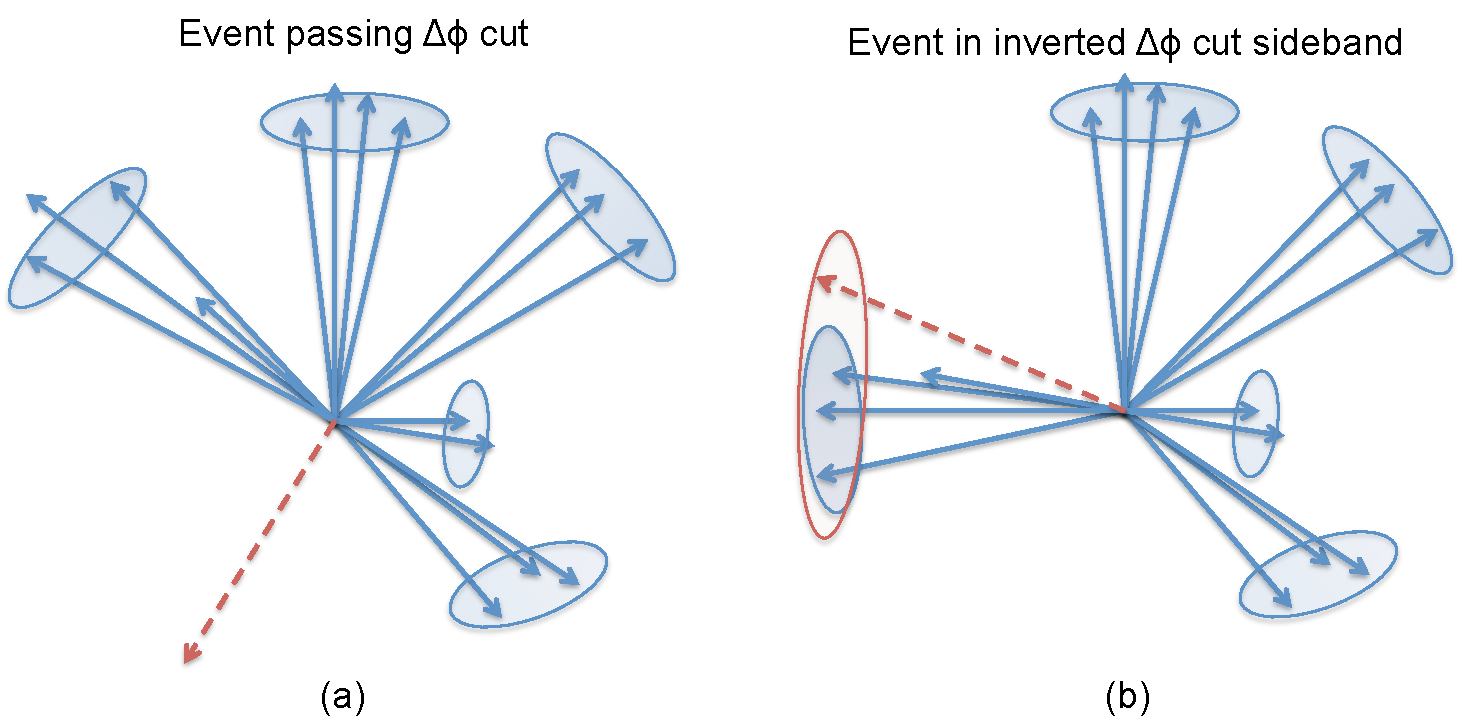
\includegraphics[width=0.59\textwidth]{sections/mc4/Backgrounds/QCD/figures/84sb/DPhiEventVsFlipDPhiEvent.pdf}
\end{center}
\caption{(a) Example of an event passing the 
$\Delta\phi_{\mathrm{jets~and}~\MET}$ cut. $\MET$ is well separated from the 
leading three jets. (b) Example of an event failing the 
$\Delta\phi_{\mathrm{jets~and}~\MET}$ cut. $\MET$ is well aligned with one of the 
leading jets and most likely arises from jet mismeasurement.}
\label{fig:deltaPhi}
\end{figure}

Although the contribution of QCD multijet events is not negligible in this 
control sample, it is still far from dominant.
MC studies in the Fig.~\ref{fig:BasicCheckQCD} show the non-QCD background contribution to the 
control sample.
%% CS check for QCD
\begin{figure}[hp]
\begin{center}
\begin{tabular}{cc}
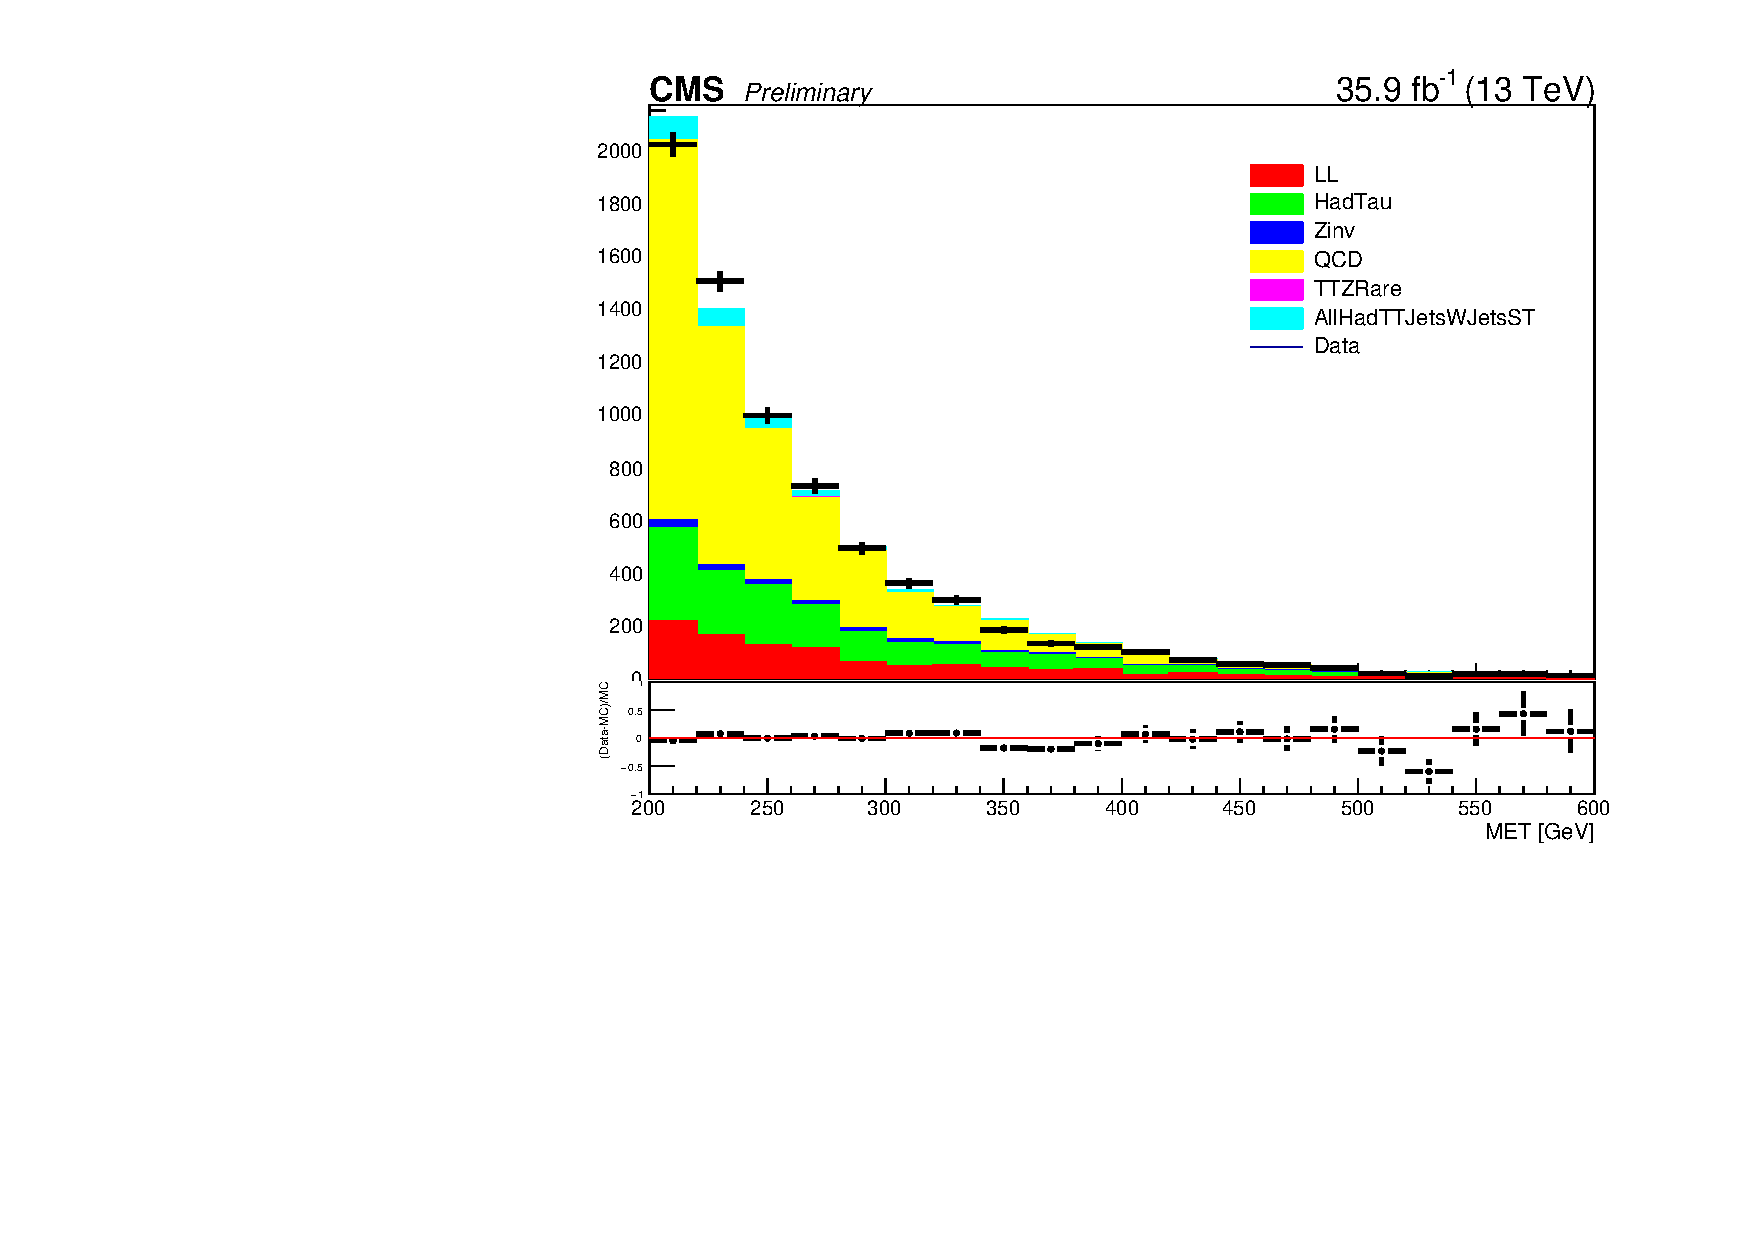
\includegraphics[width=0.49\textwidth]{sections/mc4/Backgrounds/QCD/figures/84sb/_met_BasicCheck.pdf}\\
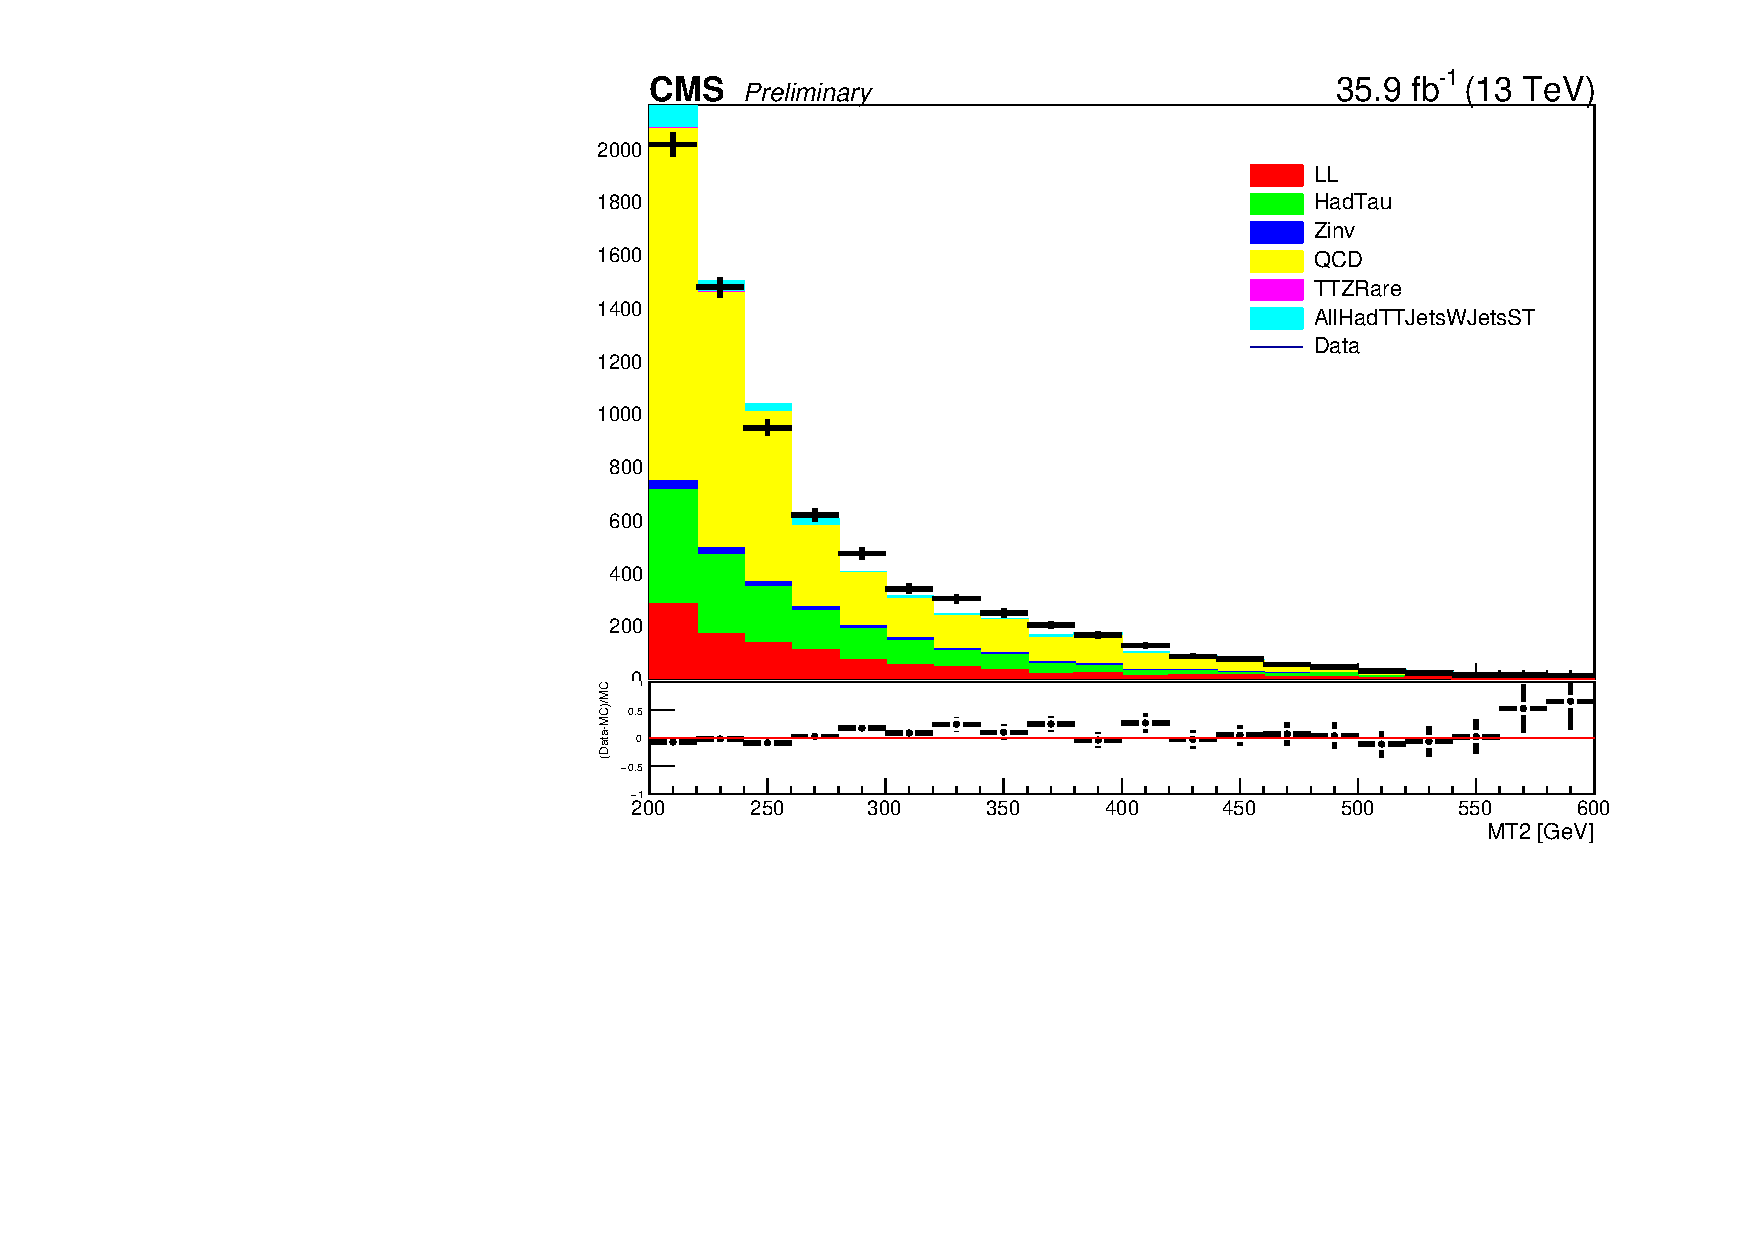
\includegraphics[width=0.49\textwidth]{sections/mc4/Backgrounds/QCD/figures/84sb/_mt2_BasicCheck.pdf}
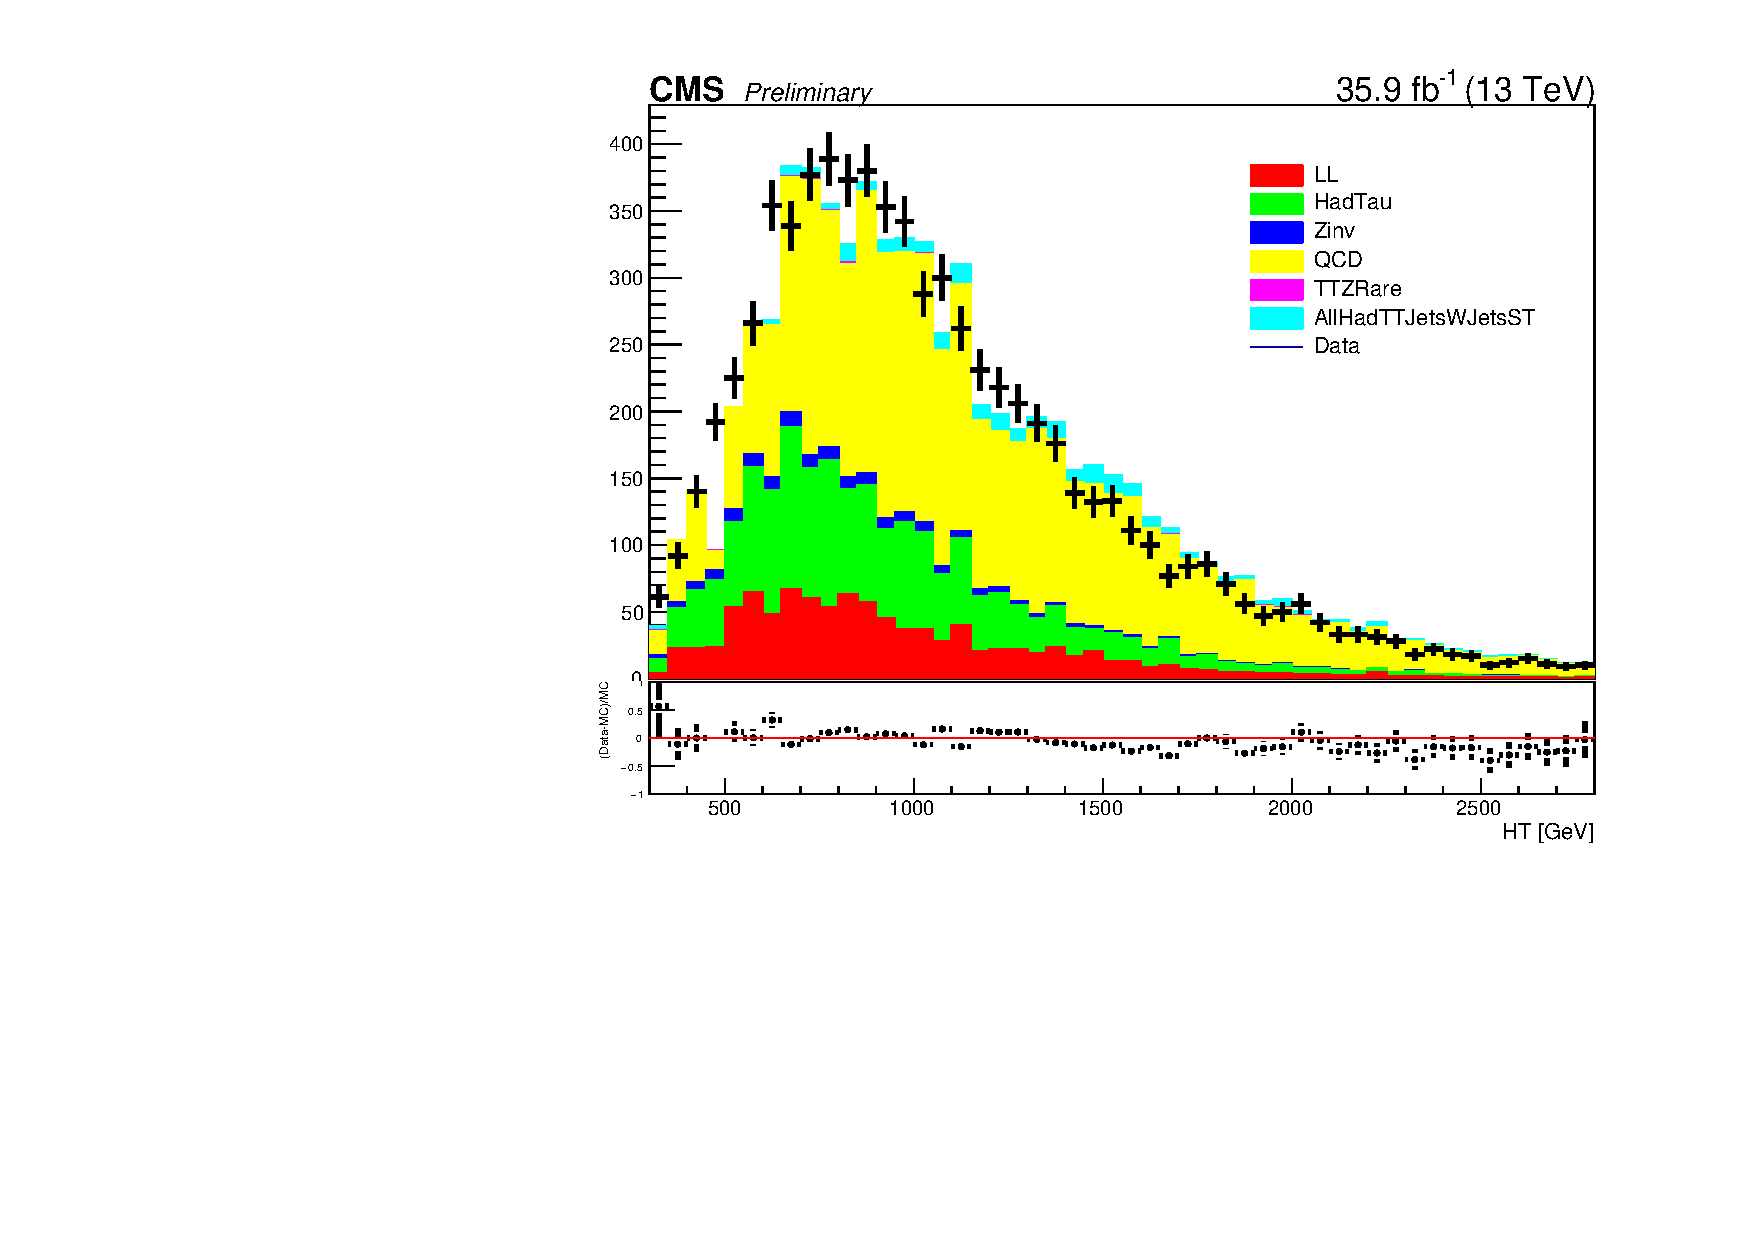
\includegraphics[width=0.49\textwidth]{sections/mc4/Backgrounds/QCD/figures/84sb/_ht_BasicCheck.pdf}\\
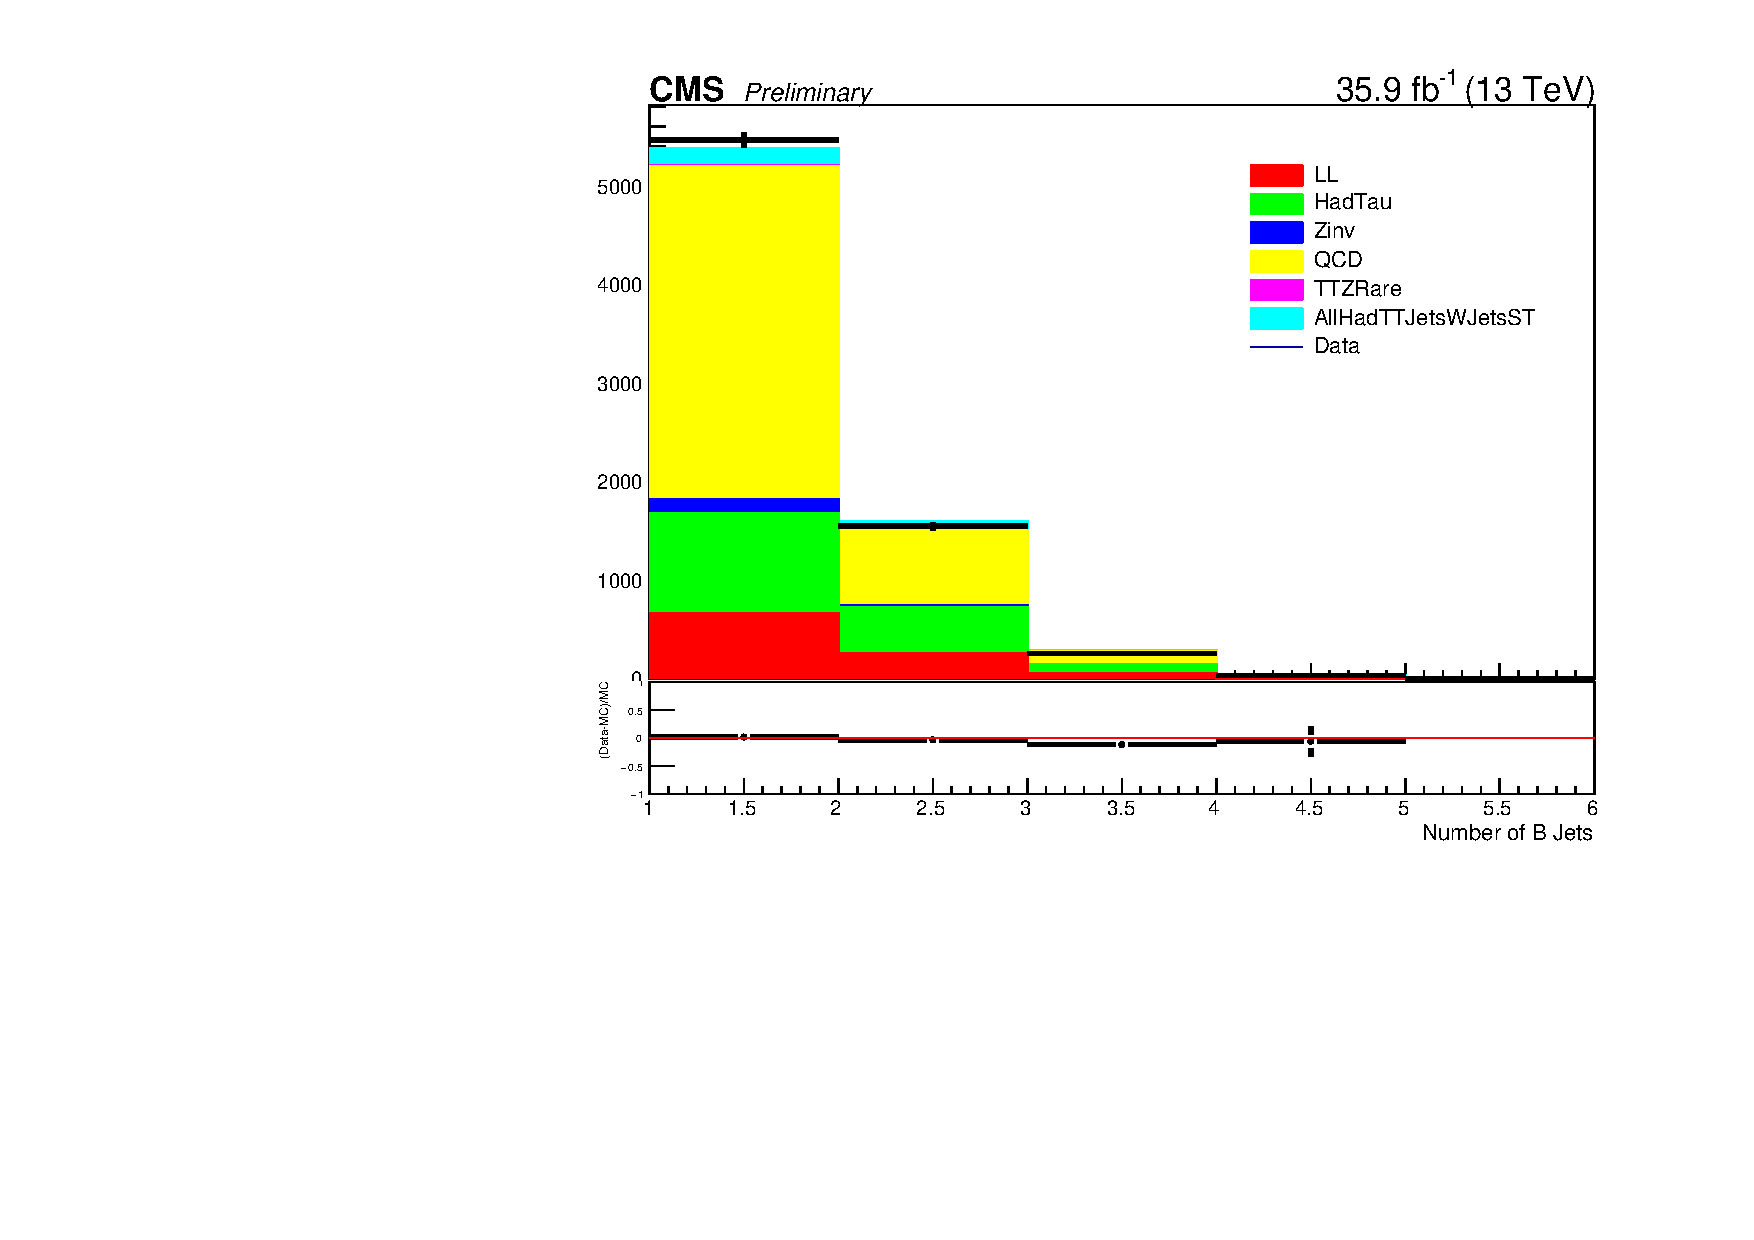
\includegraphics[width=0.49\textwidth]{sections/mc4/Backgrounds/QCD/figures/84sb/_nbjets_BasicCheck.pdf}
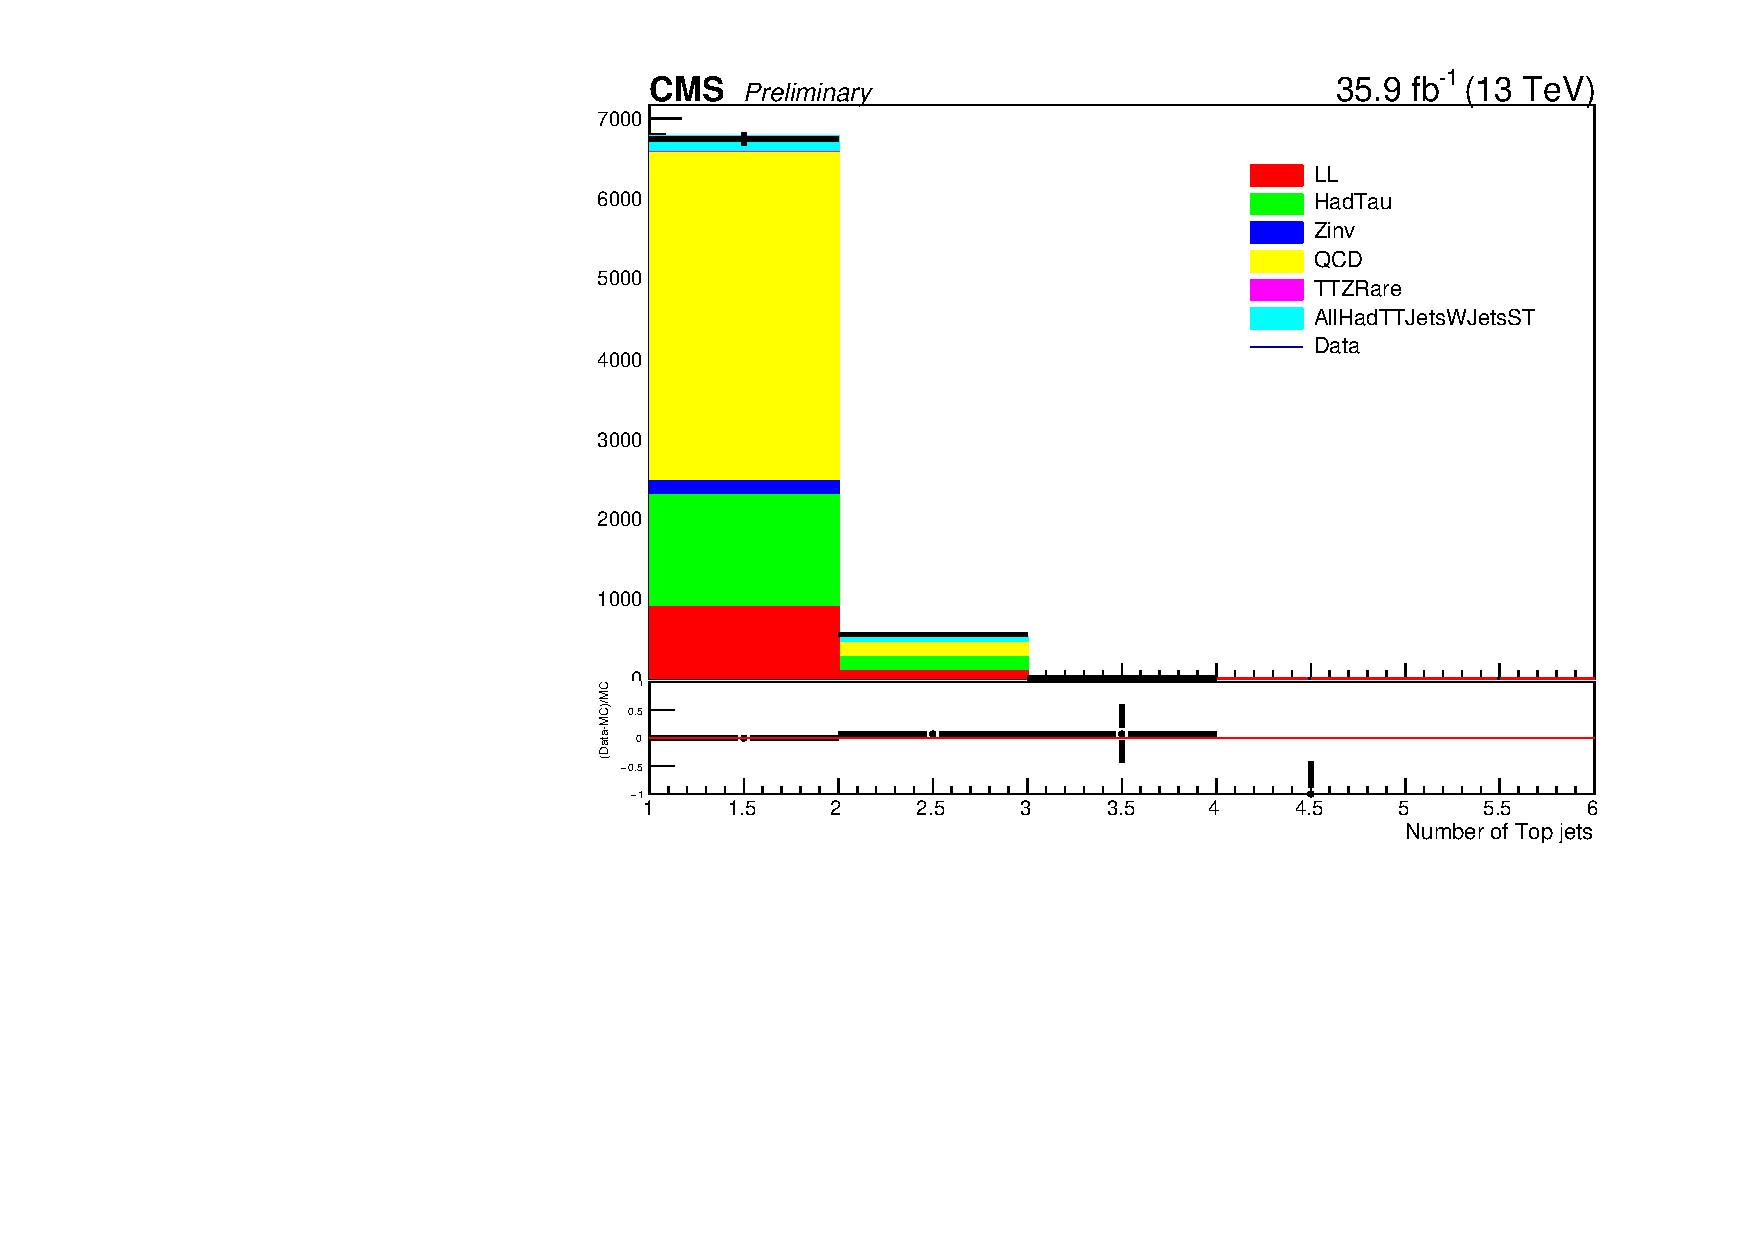
\includegraphics[width=0.49\textwidth]{sections/mc4/Backgrounds/QCD/figures/84sb/_ntopjets_BasicCheck.pdf}
\end{tabular}
\end{center}
\caption{Basic kinematic distributions in the QCD control sample. The uncertainty relates to the total
statistical uncertainty. The variables are \MET on top, \MTTwo (left) and \HT (right) in middle
and number of b-jets (left) and number of top candidates (right) on bottom.}
\label{fig:BasicCheckQCD}
\end{figure}

To assume that the events in the sideband sample are all QCD multijet events 
would lead to a gross overestimation of the total QCD background, after the 
translation factor is applied. Therefore we predict and subtract the 
contributions from lost leptons (LL), hadronic $\tau$'s (\tauh), 
and $Z$+jets ($Z\rightarrow \nu\nu$) processes from the number of data 
events counted in the inverted $\Delta\phi_{\mathrm{jets~and}~\MET}$ sample.
The remaining events make up the QCD contribution, $N^{\Delta\bar{\phi}}_{QCD}$,
is calculated as:

\begin{equation}
N^{\Delta\bar{\phi}}_{QCD} = N^{\Delta\bar{\phi}}_{Data} - N^{\Delta\bar{\phi}}_{LL} - N^{\Delta\bar{\phi}}_{\tauh} - N^{\Delta\bar{\phi}}_{Z\rightarrow \nu\nu} \; ,
\label{eq:Nqcd}
\end{equation}

where $N^{\Delta\bar{\phi}}_{X}$ is the number of type X events in the 
inverted $\Delta\phi_{\mathrm{jets~and}~ \MET}$ sideband. The contributions 
$N^{\Delta\bar{\phi}}_{LL}$, $N^{\Delta\bar{\phi}}_{\tauh}$ and 
$N^{\Delta\bar{\phi}}_{Z \rightarrow \nu\nu}$ are estimated using the same 
methods as described in the previous sections. 

The translation factor, $T_{QCD}^{MC}$, is defined as the ratio of the MC
predictions for the $\Delta\phi$ and $\Delta\bar{\phi}$ samples: 

\begin{equation}
%T_{QCD}^{MC} = \frac{N^{\Delta\phi}_{MC-QCD}}{N^{\Delta\bar{\phi}}_{MC-QCD}}= \frac{N^{\Delta\phi}_{MC} - N^{\Delta\phi}_{MC-LL} - N^{\Delta\phi}_{MC-\tauh} - N^{\Delta\phi}_{MC-Z\rightarrow \nu\nu}}{N^{\Delta\bar{\phi}}_{MC} - N^{\Delta\bar{\phi}}_{MC-LL} - N^{\Delta\bar{\phi}}_{MC-\tauh} - N^{\Delta\bar{\phi}}_{MC-Z\rightarrow \nu\nu}} \; ,
T_{QCD}^{MC} = \frac{N^{\Delta\phi}_{MC-QCD}}{N^{\Delta\bar{\phi}}_{MC-QCD}} \; ,
\label{eq:TqcdMC}
\end{equation}

while the final QCD background prediction in the search regions is calculated as:

\begin{equation}
N^{SR}_{QCD} = N^{\Delta\bar{\phi}}_{QCD} \times T_{QCD}^{Scale} \; ,
\label{eq:QCDformula}
\end{equation}

where $N^{\Delta\bar{\phi}}_{QCD}$ comes from data (as defined in Eq.~\ref{eq:Nqcd}). And the $T_{QCD}^{Scale}$ is the
$T_{QCD}^{MC}$ normalized to a translation factor measured in the 200 GeV $<\MET<$ 250 GeV sideband from data.
This normalization provides a more accurate
estimation of the true translation factors because although we trust (within the assigned uncertainties)
the shape of the MC distributions utilized to calculate them, we do not
trust their absolute values, which are corrected using the low 
200 GeV $<\MET<$ 250 GeV sideband $T_{QCD}^{Data}$ measurement. Technically 
speaking, the $T_{QCD}^{Scale}$ is based on MC only in what relates to 
its dependence on the search variables (shape), and based on data in what
relates to its normalization.

The procedure to derive the translation factors is the following:
\begin{itemize}
\item Calculate $T_{QCD}^{MC}$ from QCD MC
\item Measure $T_{QCD}^{Data}$ from Data in low $\MET$ sideband
\item Measure $T_{QCD}^{Scale}$ by normalizing the $T_{QCD}^{MC}$ versus \MET functions using the sideband 
$T_{QCD}^{Data}$ factors measured in real data from the 
200 GeV $<\MET<$ 250 GeV bin.
\end{itemize}

To summarize, we have three sets of translation factors: 
\begin{itemize}
\item \textbf{MC $T_{QCD}^{MC}$,} calculated from QCD MC and
used to evaluate the non-closure systematic uncertainty
\item \textbf{Scaled $T_{QCD}$, i.e., $T_{QCD}^{Scale}$} are factors 
applied to get final QCD background predictions.
\end{itemize}

$T_{QCD}^{MC}$'s are shown in Fig.~\ref{fig:TfactorPreFit} and Table~\ref{tab:TfactorPreFitExt}
(QCD HT-binned MC samples). The error bars are statistical uncertainties only.
%% QCD TFactor MC
\begin{figure}[htbp]
\begin{center}
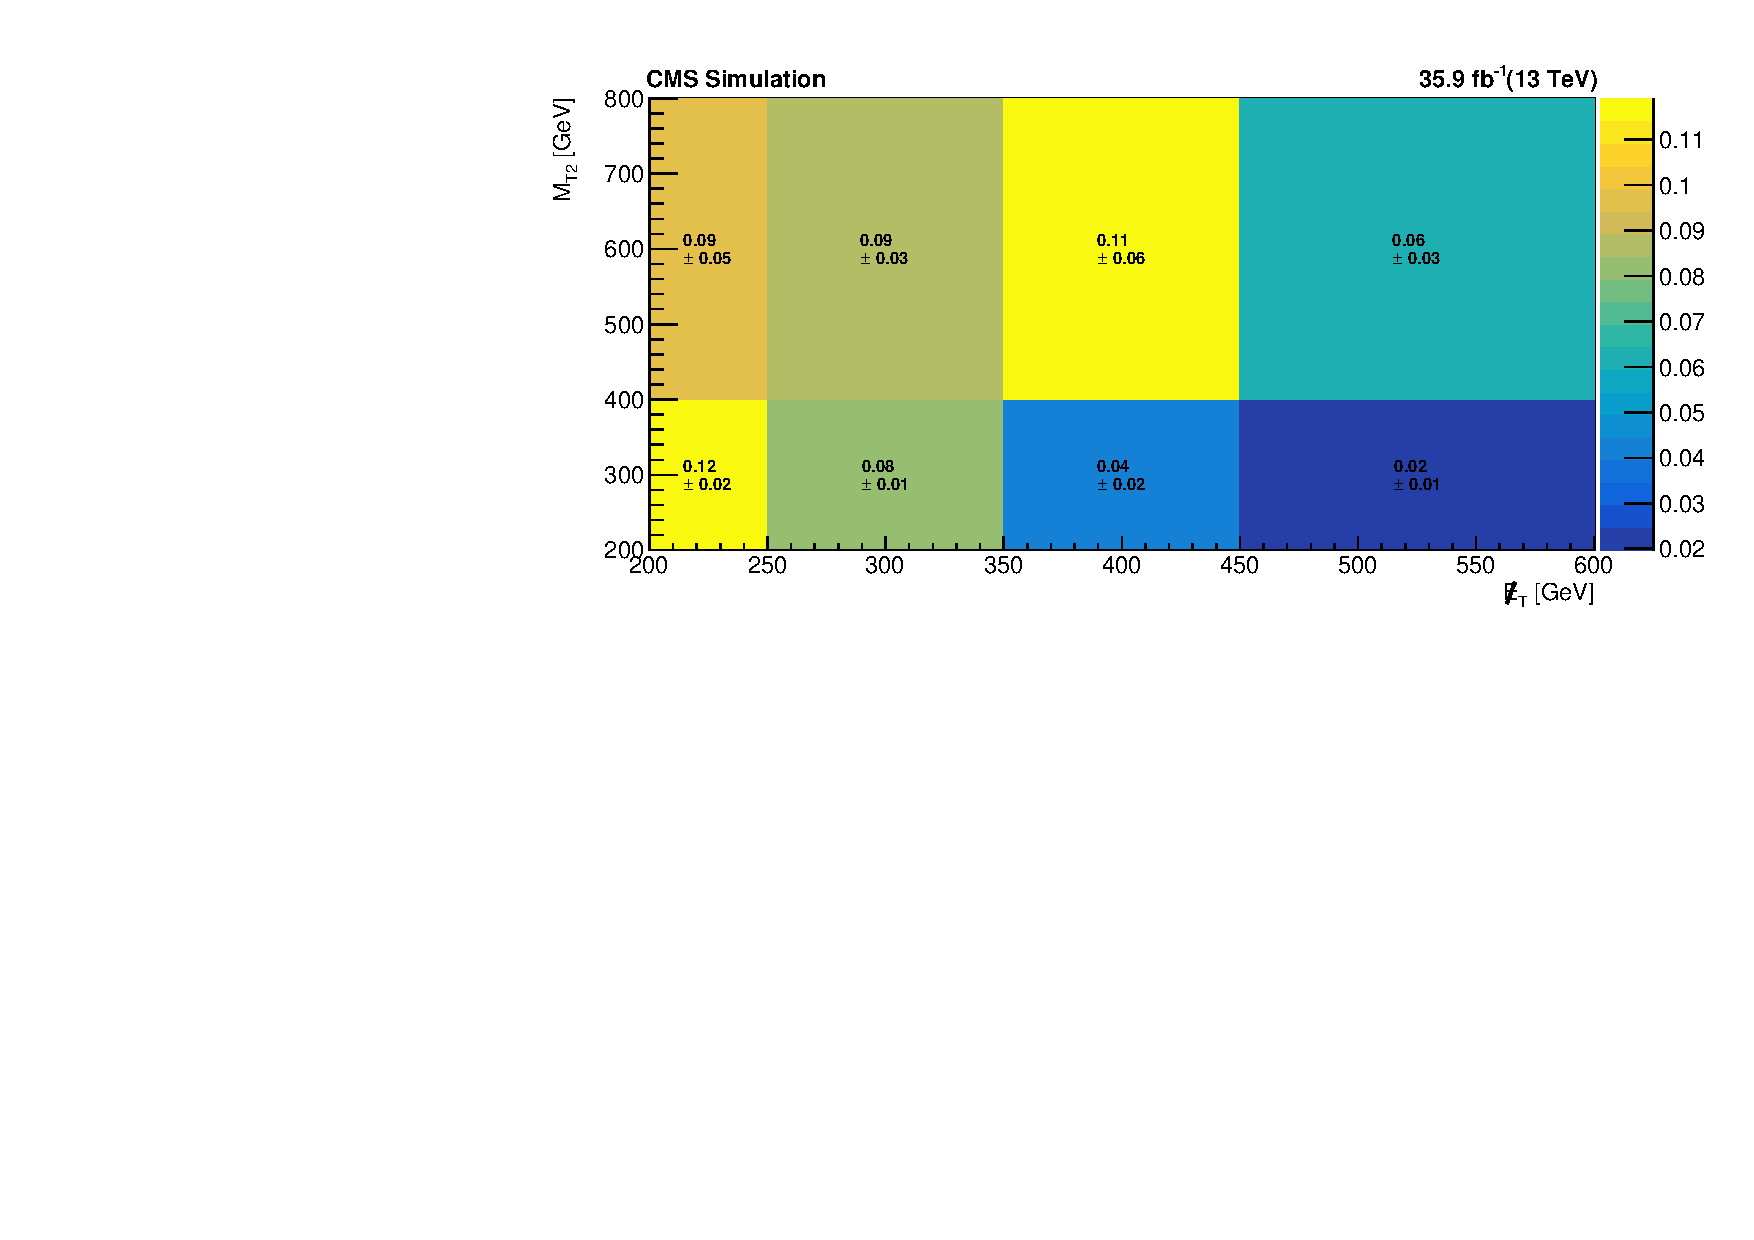
\includegraphics[width=0.89\textwidth]{sections/mc4/Backgrounds/QCD/figures/84sb/_tfactors2dPreFit.pdf}
\end{center}
\caption{ $T_{QCD}^{MC}$ versus \MET and \MTTwo distributions for \ntops and \nbjets $<$ 3 requirements. Both the 
sideband point, 200 GeV $< \MET <$ 250 GeV, and the 
signal region are included.}
\label{fig:TfactorPreFit}
\end{figure}

\begin{table}[htbp]
\fontsize{10 pt}{1.2 em}
\selectfont
\begin{centering}
\caption{\label{tab:TfactorPreFitExt} $T_{QCD}^{MC}$ versus \MET distributions for \ntops or \nbjets $>=$ 2 requirements.}
\hspace*{-4ex}
\begin{tabular}{|c|c|}
\hline
%     \MET [200,250] &          \ntops &         \nbjets &   \MTTwo or HT [GeV] &     \MET [GeV] & QCD Prediction\\
\MET [200,250] & \MET [250,Inf]\\
\hline
         0.113 &          0.095\\
\hline
\end{tabular}
\par\end{centering}
\end{table}


The low \MET $T_{QCD}^{Data}$ are measured as demonstrated in the equation from real data:
\begin{equation}
T_{QCD}^{Data} = \frac{N^{\Delta\phi}_{Data} - N^{\Delta\phi}_{MC-LL} - N^{\Delta\phi}_{MC-\tauh} - N^{\Delta\phi}_{MC-Z\rightarrow \nu\nu}}{N^{\Delta\bar{\phi}}_{Data} - N^{\Delta\bar{\phi}}_{MC-LL} - N^{\Delta\bar{\phi}}_{MC-\tauh} - N^{\Delta\bar{\phi}}_{MC-Z\rightarrow \nu\nu}} \; ,
\label{eq:TqcdData}
\end{equation}

The result of $T_{QCD}^{Scale}$ are shown in Fig.\ref{fig:TfactorScaled} and Table~\ref{tab:TfactorScaledExt}.
The low \MET scaled $T_{QCD}^{Data}$ are calculated by real data and MC with ttbar wjets and single top reweight with 84\% for now. We will move to complete data driven method for the paper.
The error bars are the total uncertainties, obtained by adding in quadrature
the statistical errors and the uncertainty coming
from the $T_{QCD}^{Data}$.
Since negative $T_{QCD}^{Scale}$ factors are not physical, we set the
background prediction to zero when this is consistent within errors.

%The only negative scale $T_{QCD}$ factor is the one in the down-right corner in Fig.\ref{fig:TfactorScaled}. 
%The negative value is around -0.0007, so it is acceptable to set it to be 0.

%% QCD TFactor Scaled
\begin{figure}[htbp]
\begin{center}
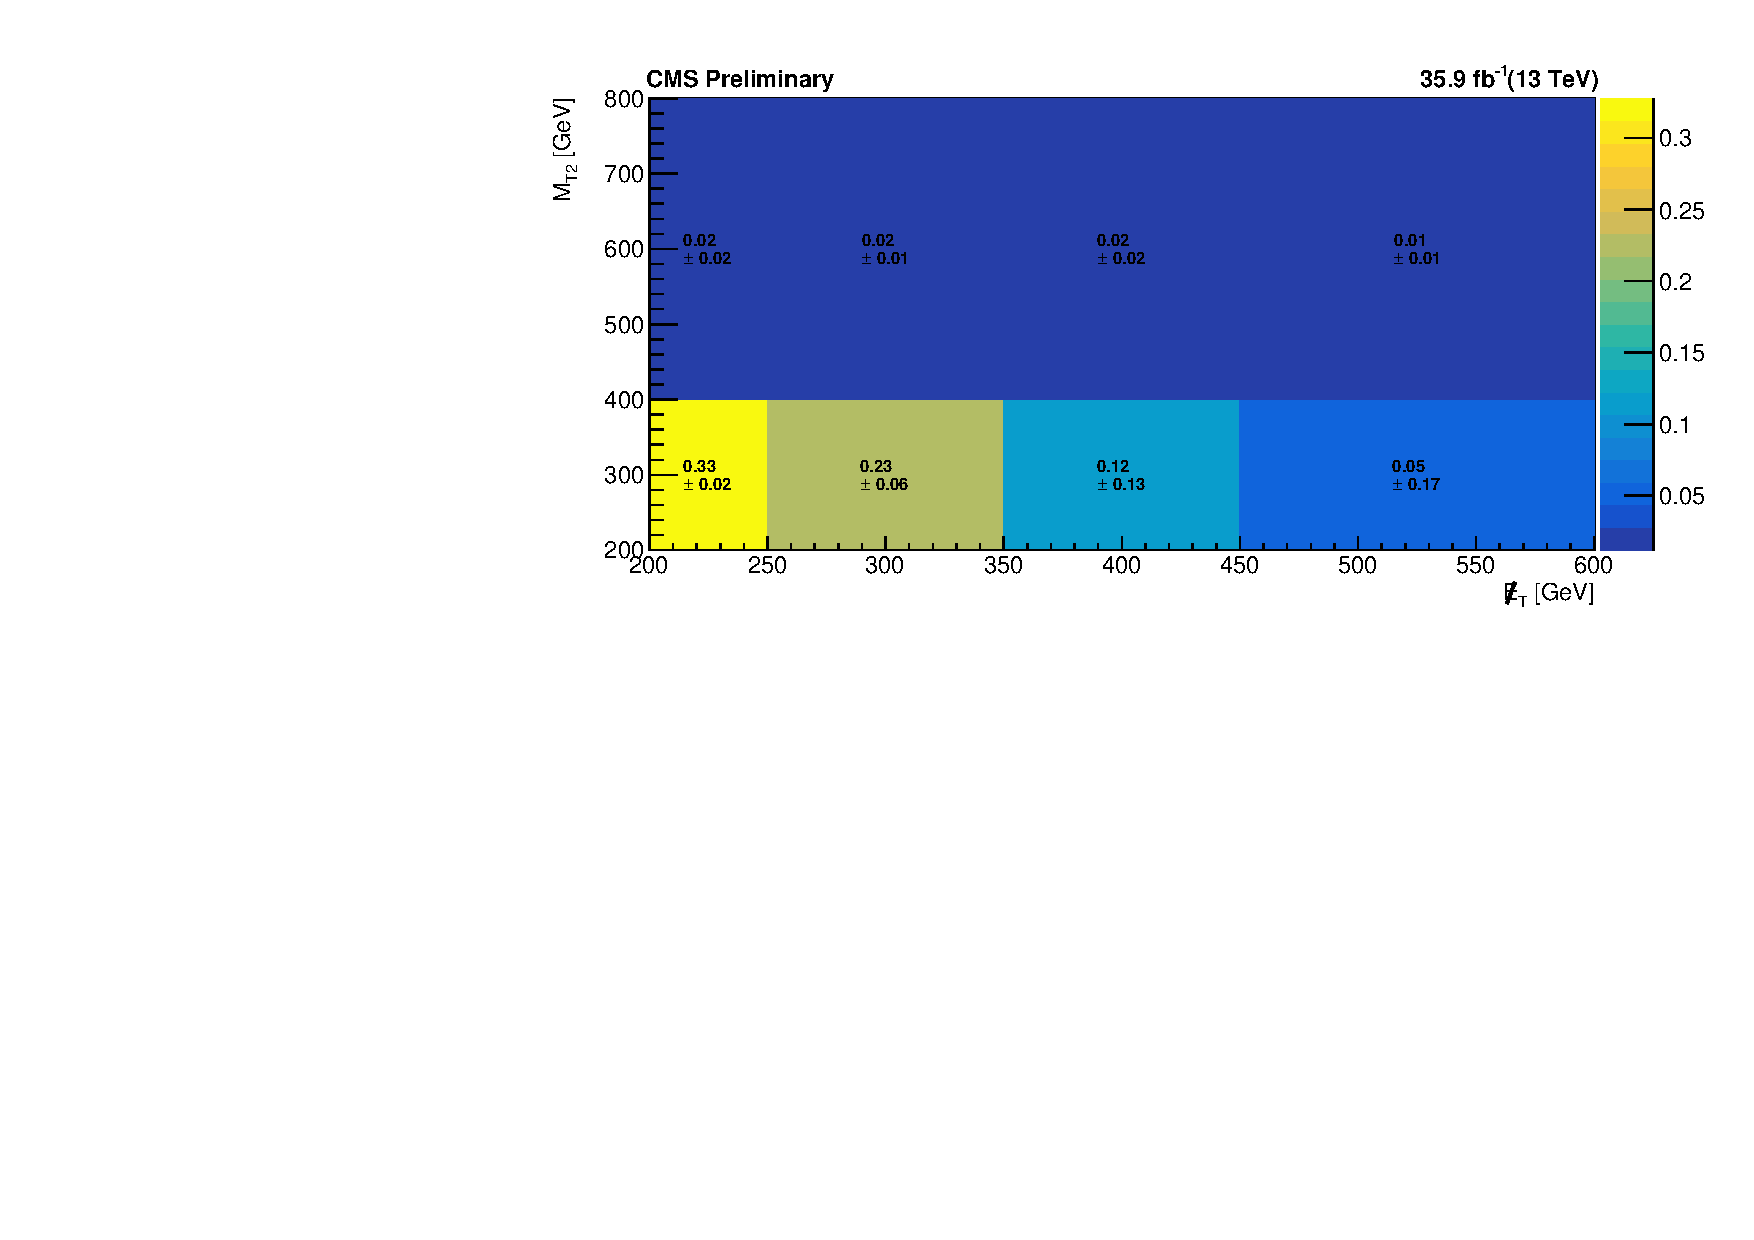
\includegraphics[width=0.89\textwidth]{sections/mc4/Backgrounds/QCD/figures/84sb/_tfactors2dScaled.pdf}
\end{center}
\caption{$T_{QCD}^{Scale}$ versus \MET and \MTTwo distributions
Both the sideband point, 200 GeV $< \MET <$ 250 GeV, and the
signal region are included.}
\label{fig:TfactorScaled}
\end{figure}

\begin{table}[htbp]
\fontsize{10 pt}{1.2 em}
\selectfont
\begin{centering}
\caption{\label{tab:TfactorScaledExt} $T_{QCD}^{Scale}$ versus \MET distributions for \ntops or \nbjets $>=$ 3 requirements.}
\hspace*{-4ex}
\begin{tabular}{|c|c|}
\hline
%     \MET [200,250] &          \ntops &         \nbjets &   \MTTwo or HT [GeV] &     \MET [GeV] & QCD Prediction\\
\MET [200,250] & \MET [250,Inf]\\
\hline
         0.312 &          0.261\\
\hline
\end{tabular}
\par\end{centering}
\end{table}

The trigger effects have been taken into account when calculating the translation factor. We measure the trigger efficiencies in low/high \HT and $\Delta\phi$/inverted $\Delta\phi$ respectively, and then apply them into translation factors calculation, both MC shape and low \MET sideband. The trigger efficiencies are showed in the Fig 2 and Fig 3.

\subsubsection{Closure Test}
The closure test is the comparison between the MC expectation after baseline and $T_{QCD}^{MC}$ prediction. It is not a circular test since we measure the $T_{QCD}^{MC}$ without binning in \ntops and \nbjets. 
The closure test aims on testing if the $T_{QCD}^{MC}$ method works on the QCD MC sample by comparing the distribution of expectation and $T_{QCD}^{MC}$ prediction in QCD MC.
As we can see in Fig.~\ref{fig:ClorureTestQCD}, closure is reasonable for all search bin variables. The non-closure uncertainty will be evaluated in the following section.
%% Closure test for QCD
\begin{figure}[hp]
\begin{center}
\begin{tabular}{cc}
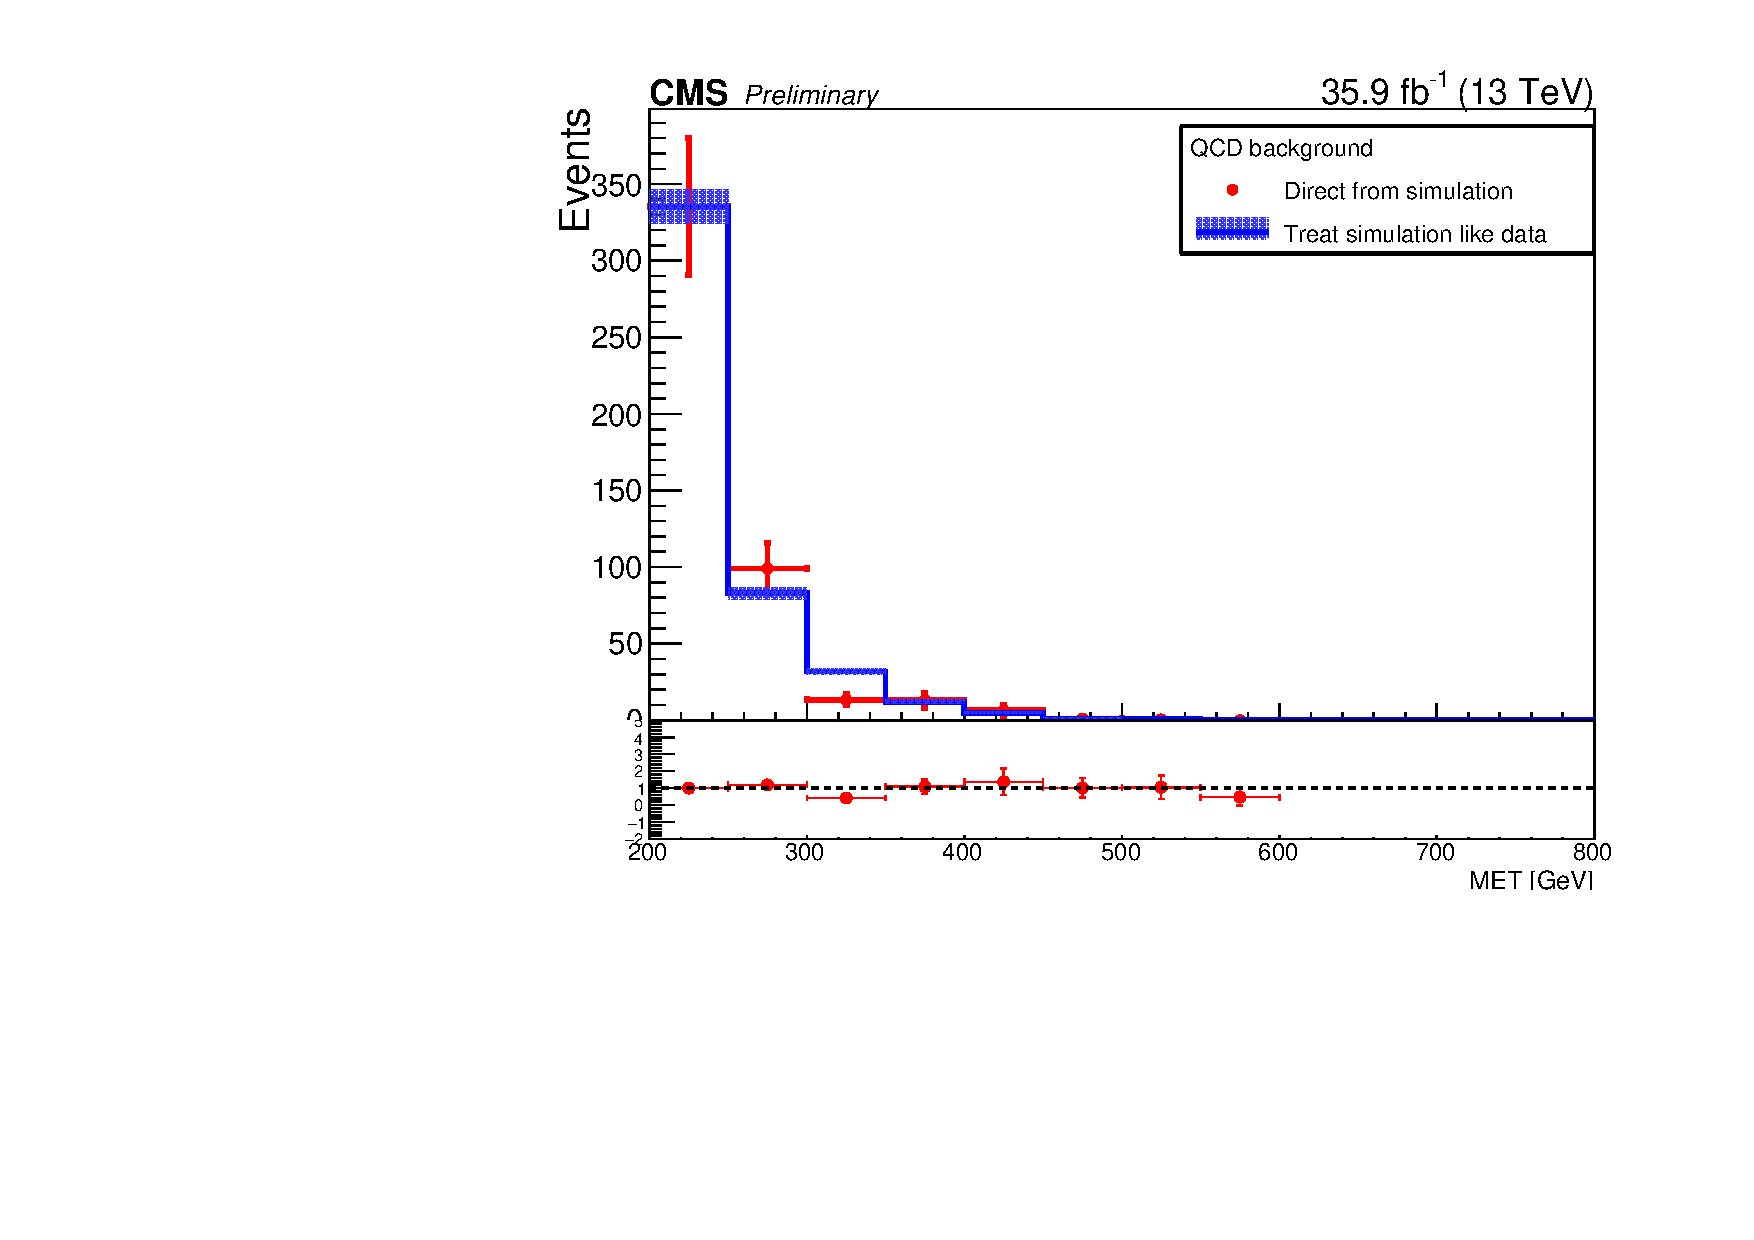
\includegraphics[width=0.49\textwidth]{sections/mc4/Backgrounds/QCD/figures/84sb/_met.pdf}\\
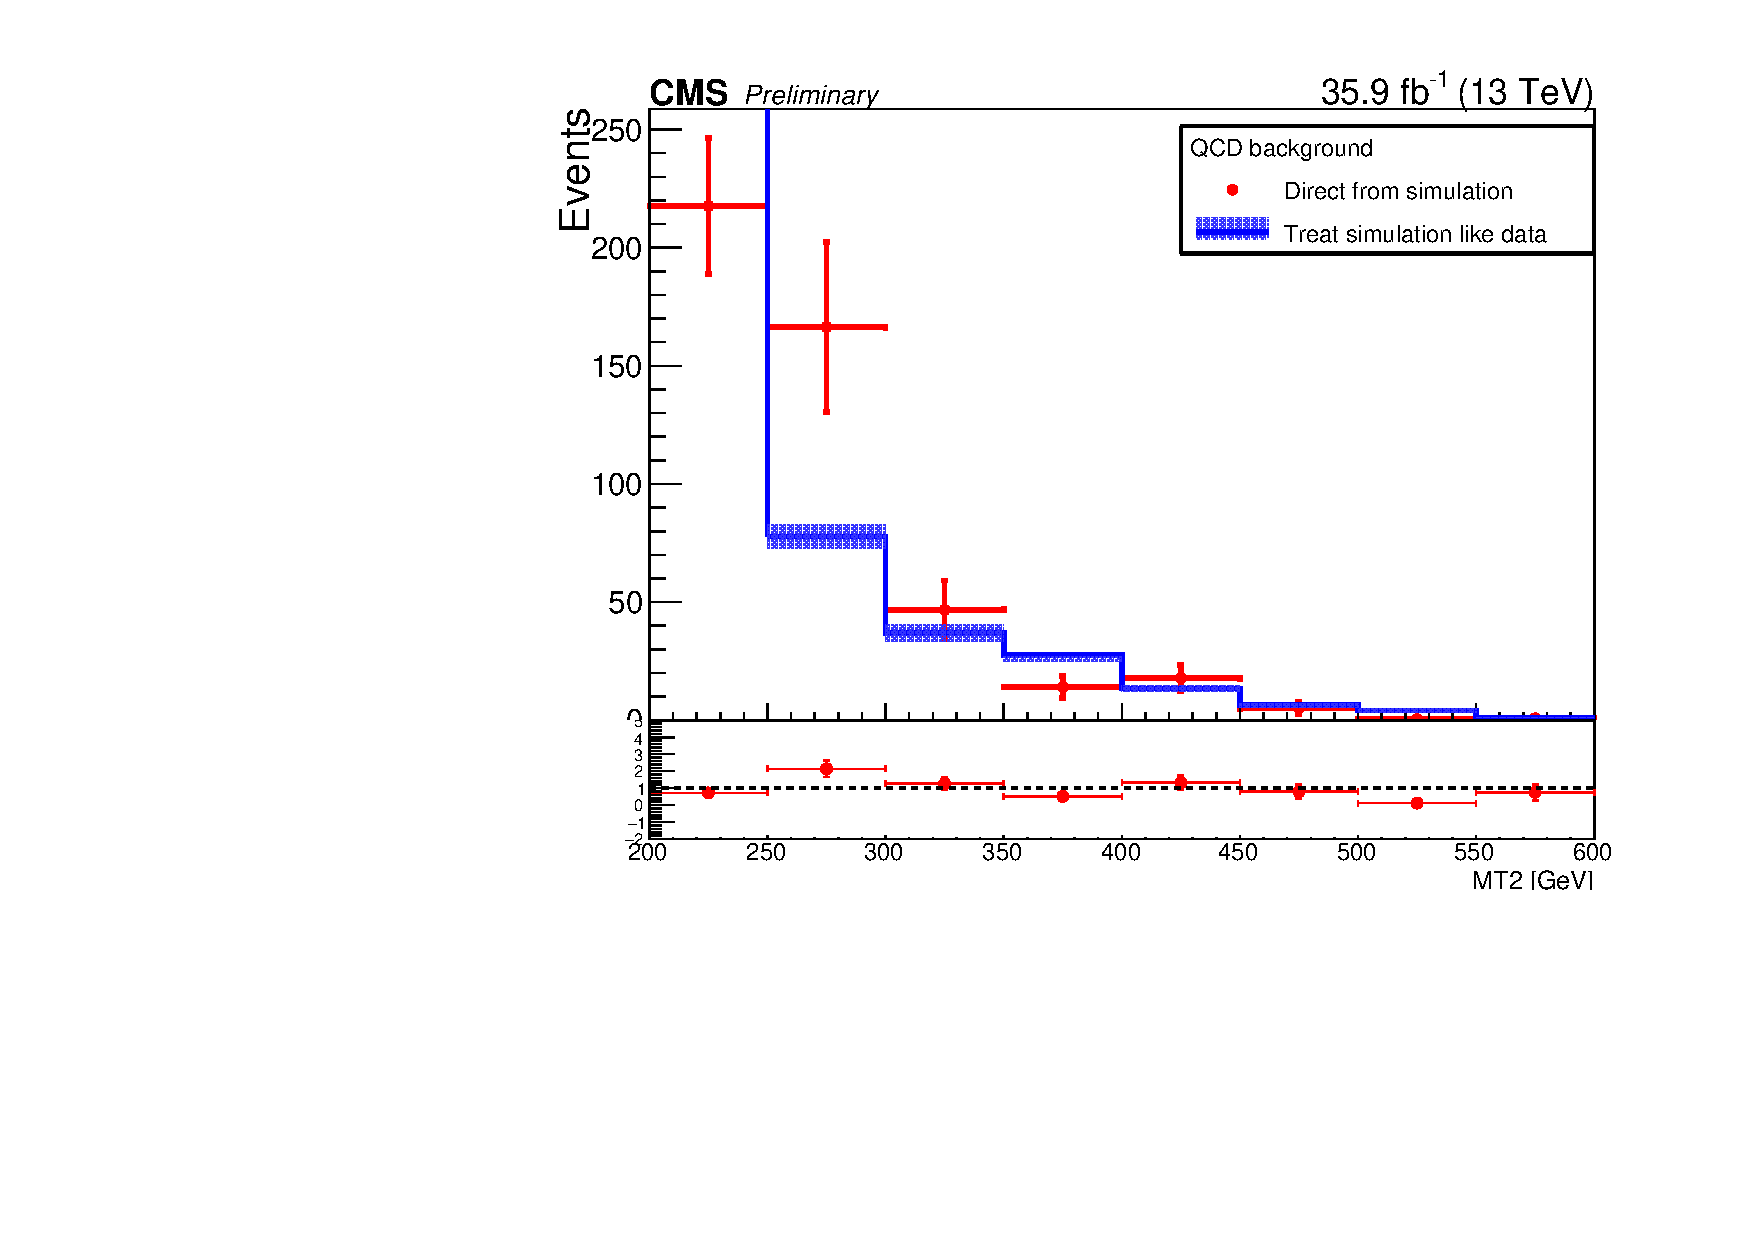
\includegraphics[width=0.49\textwidth]{sections/mc4/Backgrounds/QCD/figures/84sb/_mt2.pdf}
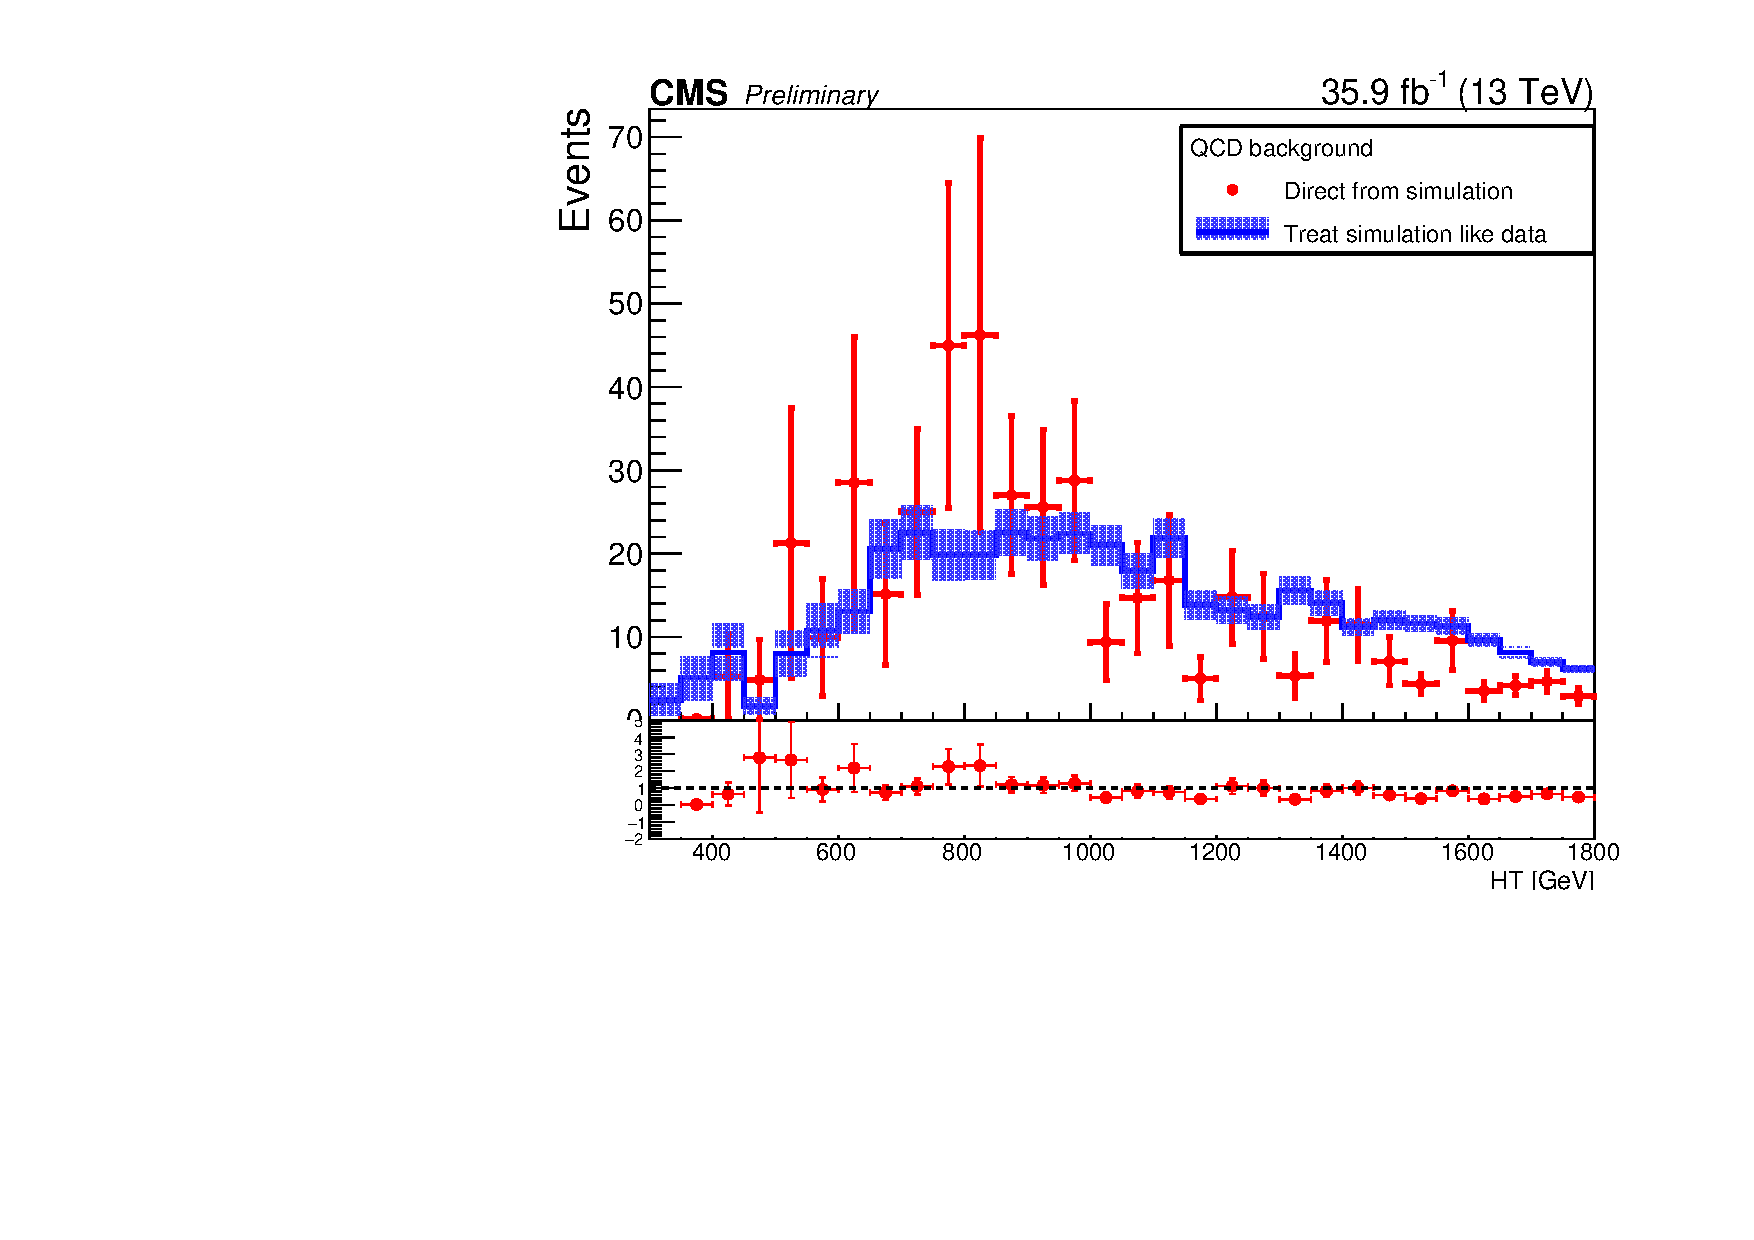
\includegraphics[width=0.49\textwidth]{sections/mc4/Backgrounds/QCD/figures/84sb/_ht.pdf}\\
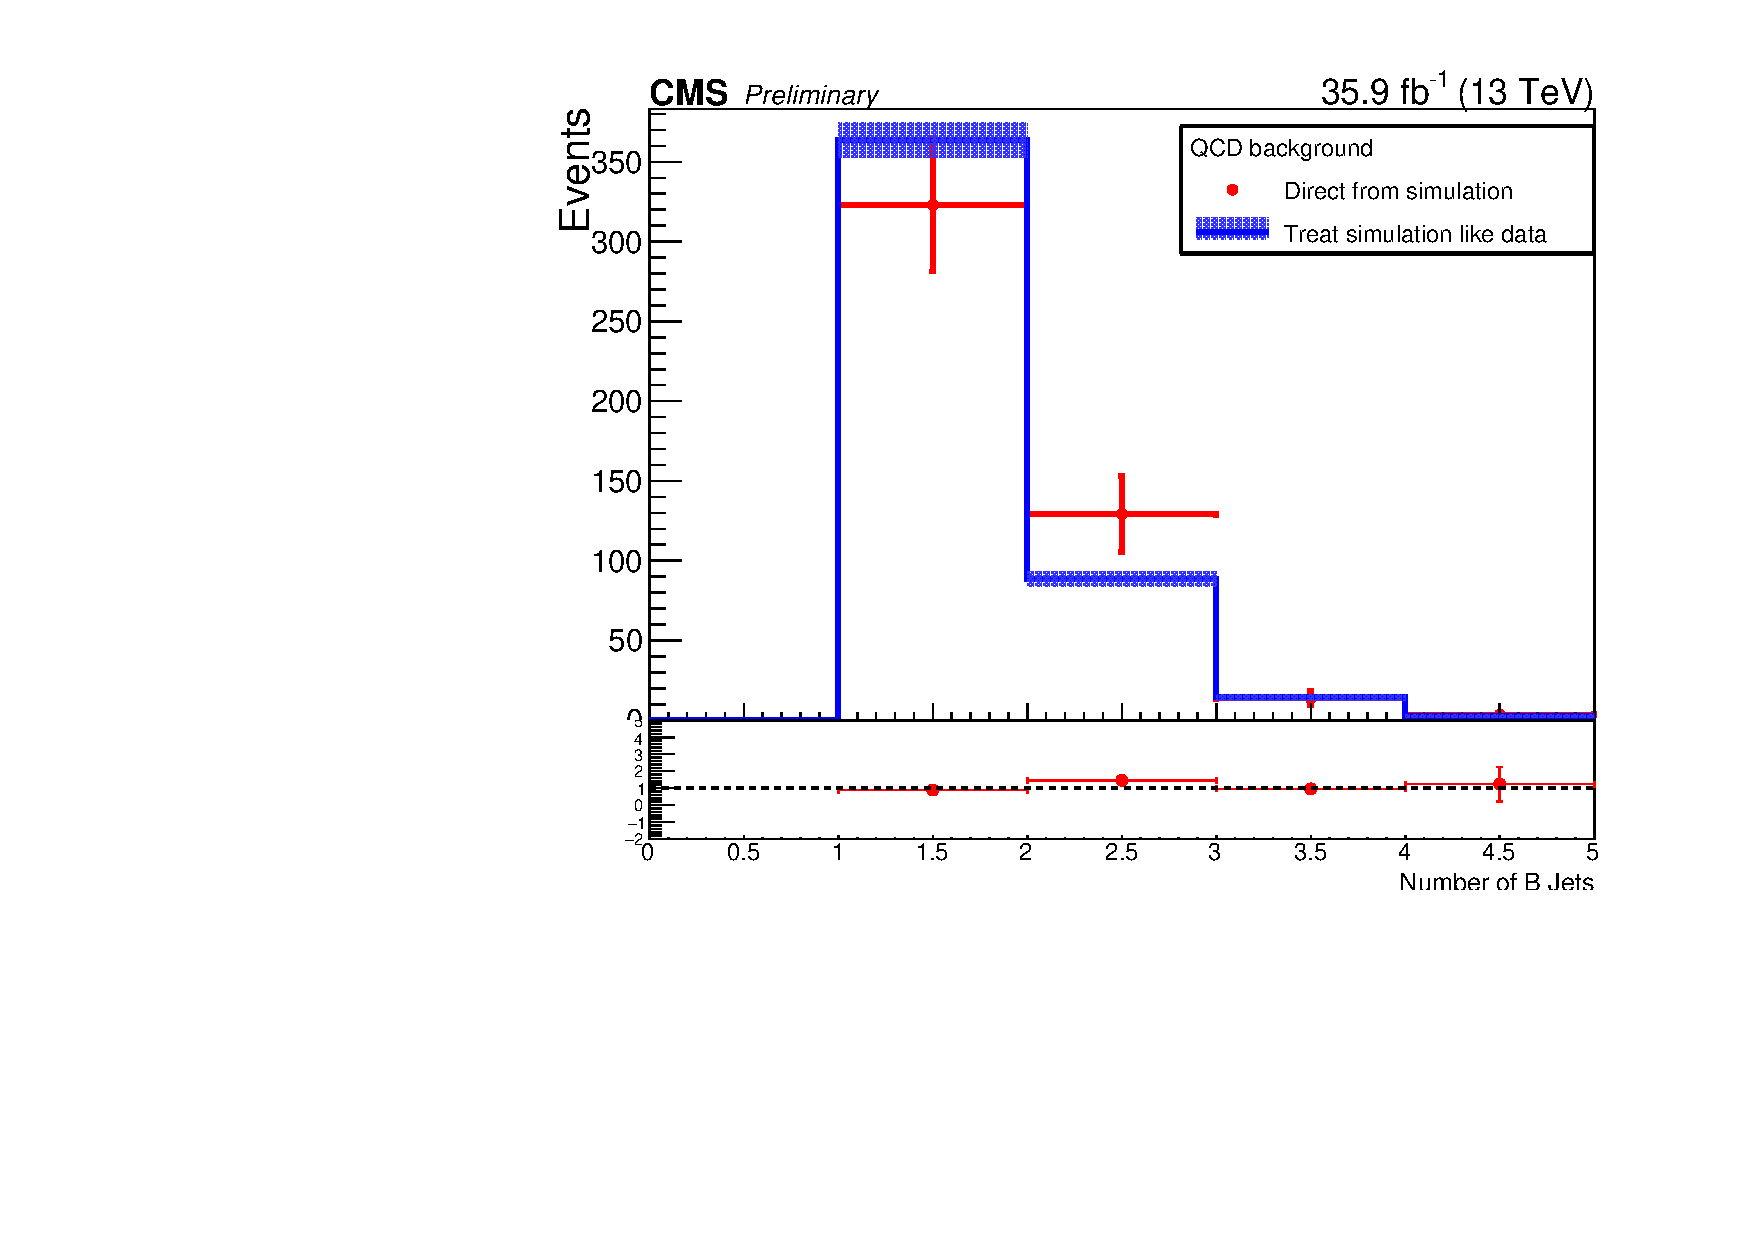
\includegraphics[width=0.49\textwidth]{sections/mc4/Backgrounds/QCD/figures/84sb/_nbjets.pdf}
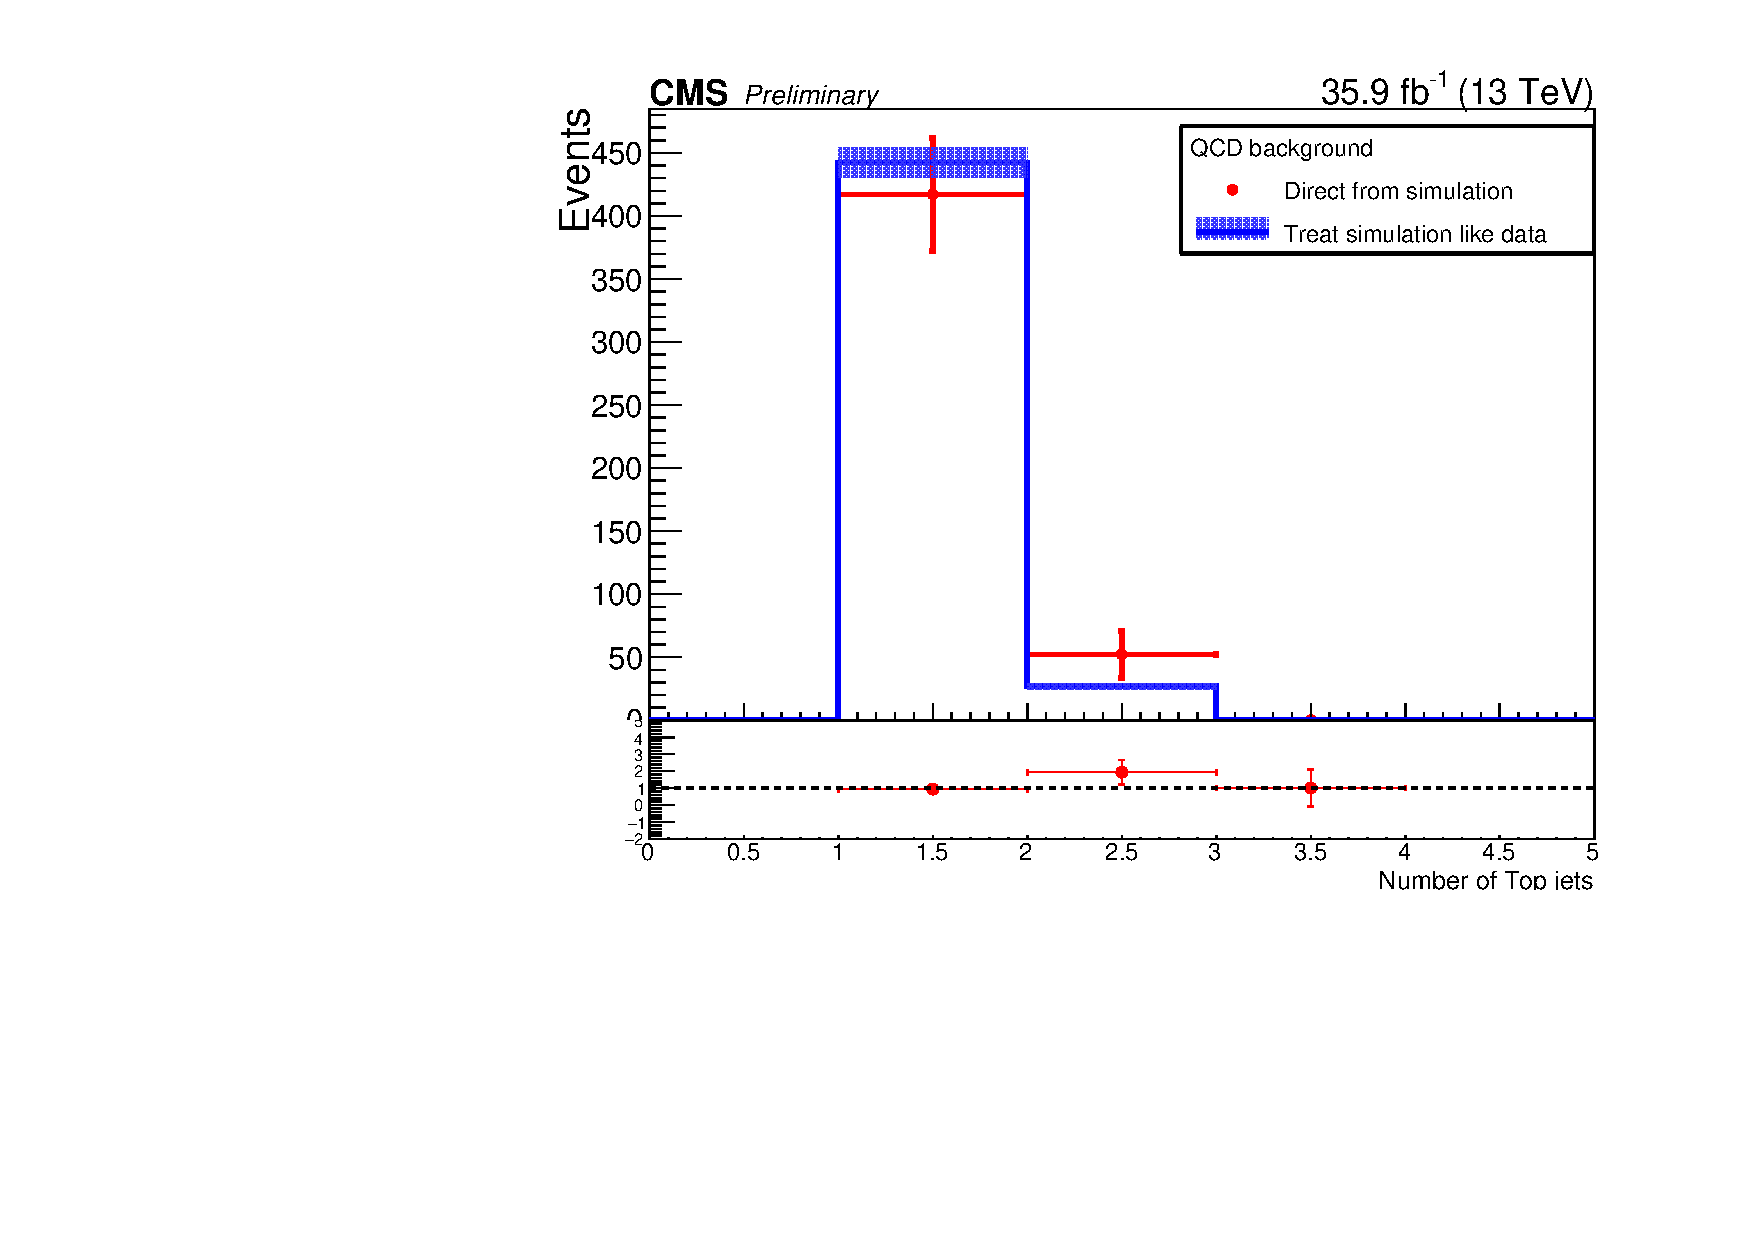
\includegraphics[width=0.49\textwidth]{sections/mc4/Backgrounds/QCD/figures/84sb/_ntopjets.pdf}
\end{tabular}
\end{center}
\caption{Closure test of the method: prediction compared to expectation in \HT
binned QCD MC samples. The uncertainty relates to the total statistical uncertainty of the prediction. 
The shown variables are \MET on top, \MTTwo (left) and \HT (right) in middle 
and number of b jets (left) and number of top jets (right) on bottom.}
\label{fig:ClorureTestQCD}
\end{figure}

QCD closure tests with $T_{QCD}^{MC}$ applied for all search bins are shown in
Fig~\ref{fig:SBClosure}. The uncertainties showed in the plot are just statistics uncertainty.
%% QCD search bin closure
\begin{figure}[htbp]
\begin{center}
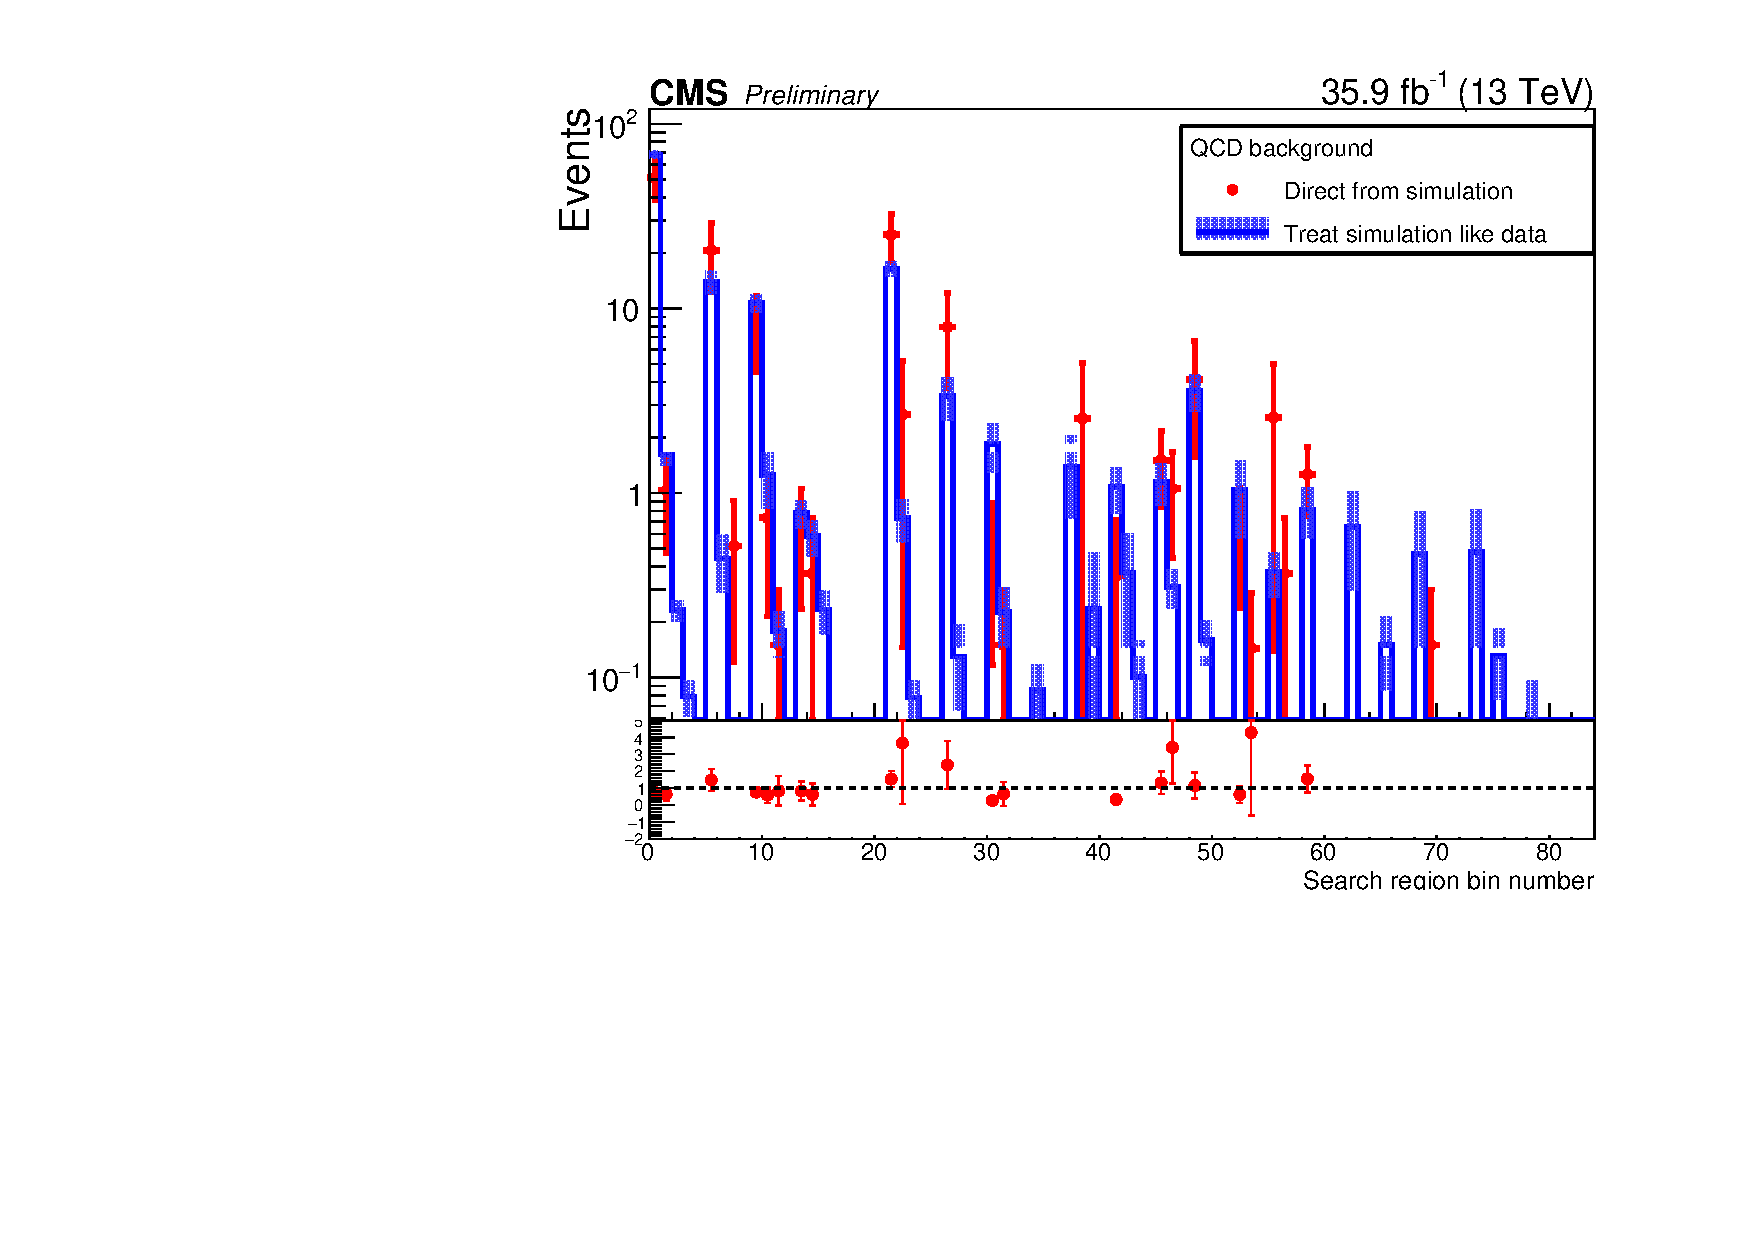
\includegraphics[width=0.89\textwidth]{sections/mc4/Backgrounds/QCD/figures/84sb/_sb.pdf}
\end{center}\caption{QCD background Closure tests in all search bins with $T_{QCD}^{MC}$.}
\label{fig:SBClosure}
\end{figure}

\subsubsection{Systematic Uncertainties}

The sources of QCD background systematical uncertainty are:

\begin{itemize}
\item \textbf{$T_{QCD}^{Scale}$}
\item \textbf{Non-closure}
\item \textbf{Contamination from other backgrounds}
%\item \textbf{Trigger efficiency}
\end{itemize}

\paragraph{$T_{QCD}^{Scale}$ uncertainties}
The uncertainty of $T_{QCD}^{Scale}$ factors are the statistical uncertainty when we calculate $T_{QCD}^{MC}$ and $T_{QCD}^{Data}$.

\paragraph{Non-Closure uncertainty}

For the evaluation of the systematic uncertainty, the prediction is 
derived from $T_{QCD}^{MC}$'s. 
The expectations and predictions are compatiable in 
most of the search bins. In the case of the bins without enough ($<4$) expected MC events,
we take the uncertainties from \MET and  \MTTwo or \MET and  \HT 2 dimensional inclusive closure plots, then combine with 1 dimensional \ntops and \nbjets closure in quardrature. If no enough MC statistics in \MET and  \MTTwo or \MET and  \HT 2 dimensional inclusive closure plots, we will take 4 independent closure from search bin variables inclusive closure plots then combine them in quardrature. However, we will have no MC evnets in some bins, like when \MET greater than 700 GeV, in this case, we will take the value from its neighbour. 

\paragraph{Contamination uncertainty}
Since we are using input from other background to estimate the contamination in QCD control region, we also integrate this into total systematic uncertainty.

\begin{table}[htbp]
\fontsize{10 pt}{1.2 em}
\selectfont
\begin{centering}
\caption{\label{tab:QCDpredsys} Contributions from different
sources of systematic uncertainty to the QCD background prediction.}
\hspace*{-4ex}
\begin{tabular}{|c|c|c|}
\hline
Process & Source & Effect on QCD Prediction in $\%$\\
\hline
$T_{QCD}^{Scale}$ factors & Statistical uncertainty on $T_{QCD}^{MC}$ and $T_{QCD}^{Data}$ & 30 to 330 \\
\hline
Closure & Non-closure and statistical precision of the closure & 30 to 500 \\
\hline
Contamination from other backgrounds & Uncertainties from other background input & 2 to 50 \\
\hline
\end{tabular}
\par\end{centering}
\end{table}

\subsubsection{QCD background prediction}
The QCD background predictions for the full $35.9$fb$^{-1}$ dataset in all 
search bins are shown in Fig.~\ref{fig:SBPrediction} and listed in 
Table~\ref{tab:QCDpred84_1} and Table~\ref{tab:QCDpred84_2}, which includes statistical and systematic uncertainties.
%% QCD search bin Prediction
\begin{figure}[htbp]
\begin{center}
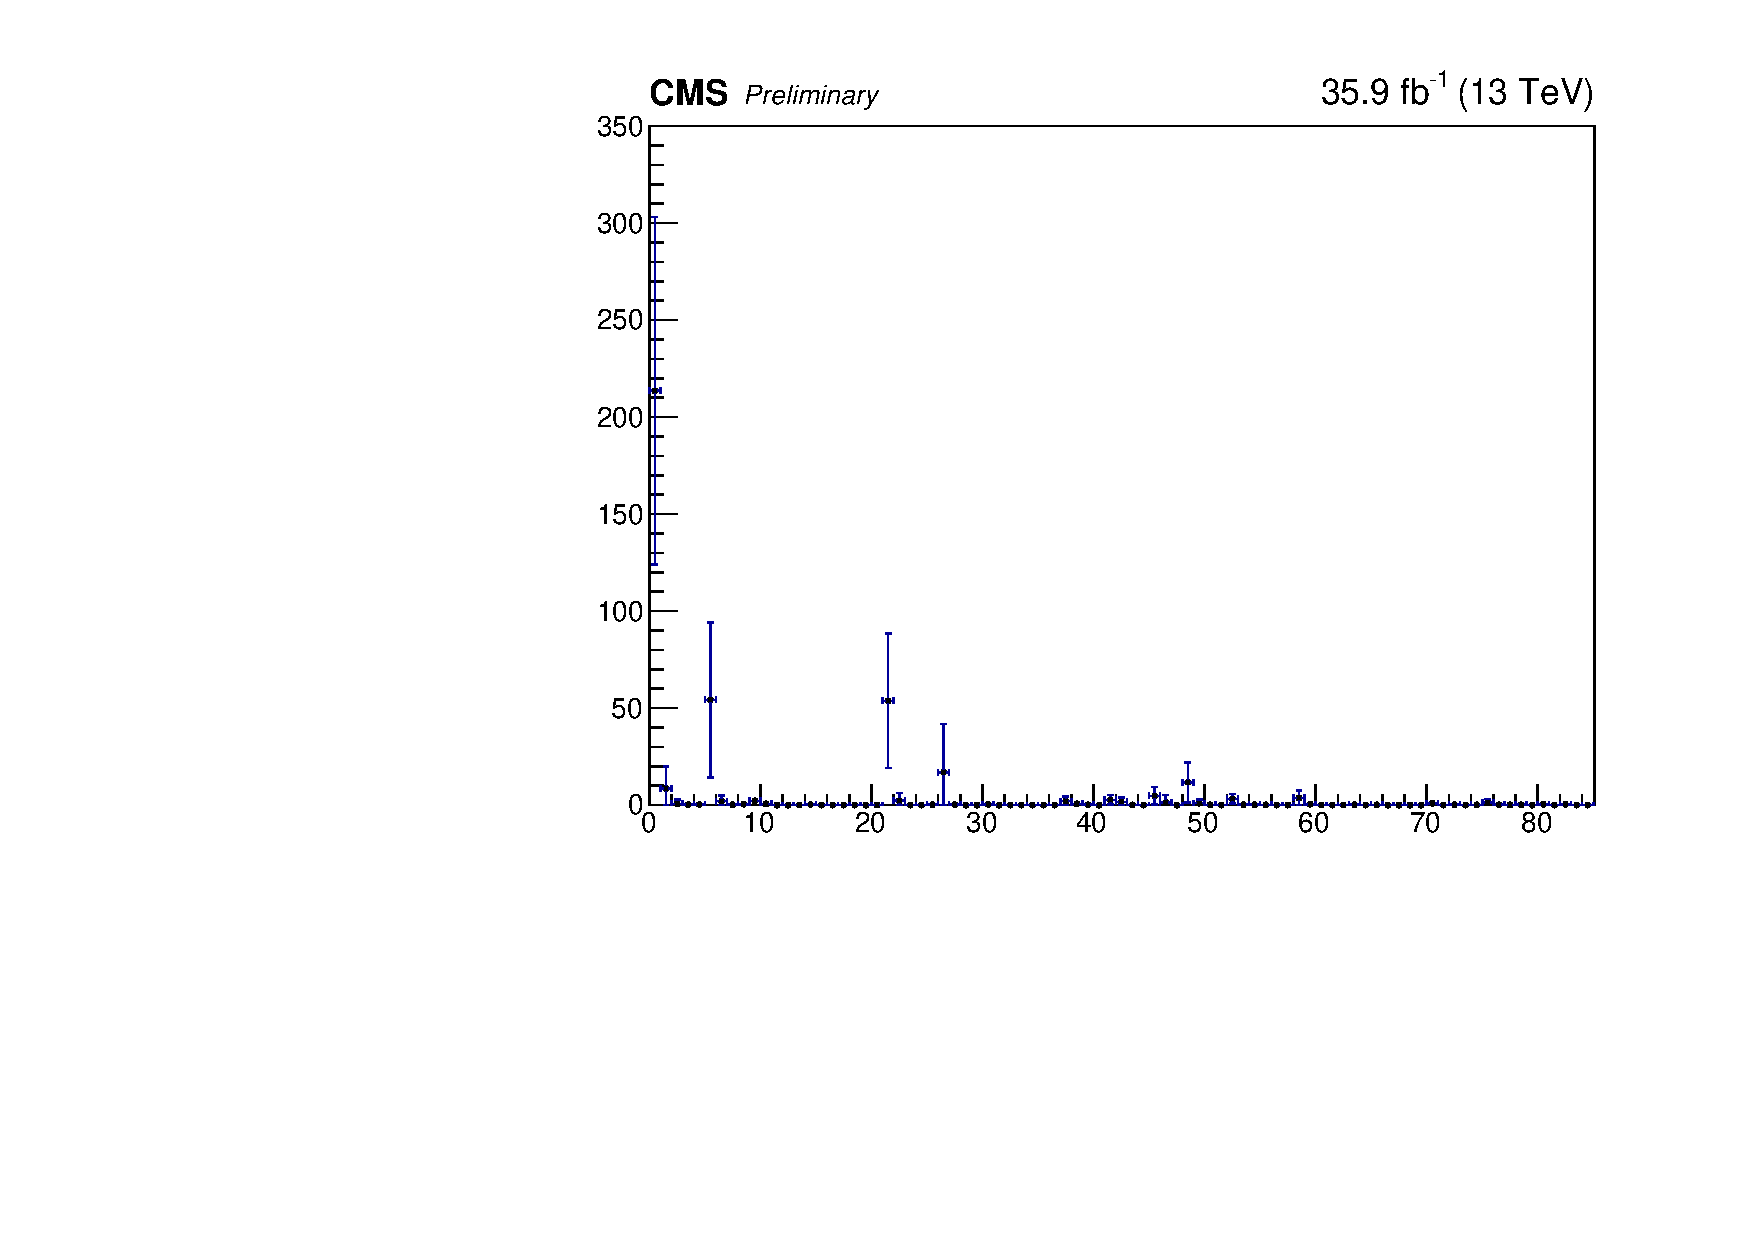
\includegraphics[width=0.89\textwidth]{sections/mc4/Backgrounds/QCD/figures/84sb/_sb_Data.pdf}
\end{center}\caption{QCD background predictions in all search bins.}
\label{fig:SBPrediction}
\end{figure}

\begin{table}[htbp]
\fontsize{10 pt}{1.2 em}
\selectfont
\begin{centering}
\caption{\label{tab:QCDpred84_1} Predicted QCD backgrounds corresponding to 
the full $35.9$~fb$^{-1}$ data sample in first 48 search bins.}
\hspace*{-4ex}
\begin{tabular}{|c|c|c|c|c||c|}
\hline
     Search Bin &          \ntops &         \nbjets &   \MTTwo [GeV] &     \MET [GeV] & QCD Prediction\\
 \hline
              0 &               1 &               1 &         200-300 &         250-400 & 213.6 $^{+8.556}_{-8.324}$  $^{+89.18}_{-89.18}$  \\
 \hline
              1 &               1 &               1 &         200-300 &         400-500 & 8.587 $^{+1.443}_{-1.318}$  $^{+11.12}_{-11.12}$  \\
 \hline
              2 &               1 &               1 &         200-300 &         500-600 & 0.644 $^{+0.339}_{-0.279}$  $^{+2.180}_{-2.180}$  \\
 \hline
              3 &               1 &               1 &         200-300 &         600-750 & 0.300 $^{+0.254}_{-0.192}$  $^{+1.031}_{-1.031}$  \\
 \hline
              4 &               1 &               1 &         200-550 &            750+ & 0.327 $^{+0.239}_{-0.176}$  $^{+1.111}_{-1.111}$  \\
 \hline
              5 &               1 &               1 &         300-400 &         250-400 & 54.22 $^{+4.673}_{-4.437}$  $^{+39.76}_{-39.76}$  \\
 \hline
              6 &               1 &               1 &         300-400 &         400-500 & 2.029 $^{+0.767}_{-0.637}$  $^{+2.842}_{-2.842}$  \\
 \hline
              7 &               1 &               1 &         300-400 &         500-600 & 0.212 $^{+0.222}_{-0.159}$  $^{+1.141}_{-1.141}$  \\
 \hline
              8 &               1 &               1 &         300-400 &         600-750 & 0.442 $^{+0.239}_{-0.176}$  $^{+1.485}_{-1.485}$  \\
 \hline
              9 &               1 &               1 &         400-550 &         250-400 & 2.214 $^{+0.250}_{-0.233}$  $^{+1.397}_{-1.397}$  \\
 \hline
             10 &               1 &               1 &         400-550 &         400-500 & 0.621 $^{+0.170}_{-0.146}$  $^{+0.640}_{-0.640}$  \\
 \hline
             11 &               1 &               1 &         400-550 &         500-600 & 0.000 $^{+0.027}_{-0.009}$  $^{+0.005}_{-0.005}$  \\
 \hline
             12 &               1 &               1 &         400-550 &         600-750 & 0.007 $^{+0.031}_{-0.015}$  $^{+0.012}_{-0.012}$  \\
 \hline
             13 &               1 &               1 &         550-750 &         250-400 & 0.061 $^{+0.060}_{-0.040}$  $^{+0.053}_{-0.053}$  \\
 \hline
             14 &               1 &               1 &         550-750 &         400-500 & 0.319 $^{+0.121}_{-0.097}$  $^{+0.388}_{-0.388}$  \\
 \hline
             15 &               1 &               1 &         550-750 &         500-600 & 0.024 $^{+0.047}_{-0.033}$  $^{+0.039}_{-0.039}$  \\
 \hline
             16 &               1 &               1 &         550-750 &         600-750 & 0.036 $^{+0.042}_{-0.028}$  $^{+0.052}_{-0.052}$  \\
 \hline
             17 &               1 &               1 &         550-750 &            750+ & 0.004 $^{+0.027}_{-0.009}$  $^{+0.007}_{-0.007}$  \\
 \hline
             18 &               1 &               1 &            750+ &         250-600 & 0.032 $^{+0.034}_{-0.019}$  $^{+0.170}_{-0.170}$  \\
 \hline
             19 &               1 &               1 &            750+ &         600-750 & 0.001 $^{+0.027}_{-0.009}$  $^{+0.009}_{-0.009}$  \\
 \hline
             20 &               1 &               1 &            750+ &            750+ & 0.055 $^{+0.042}_{-0.028}$  $^{+0.290}_{-0.290}$  \\
 \hline
             21 &               1 &               2 &         200-350 &         250-400 & 53.76 $^{+4.982}_{-4.747}$  $^{+34.32}_{-34.32}$  \\
 \hline
             22 &               1 &               2 &         200-350 &         400-500 & 2.278 $^{+0.949}_{-0.822}$  $^{+3.946}_{-3.946}$  \\
 \hline
             23 &               1 &               2 &         200-350 &         500-600 & 0.000 $^{+0.204}_{-0.139}$  $^{+0.045}_{-0.045}$  \\
 \hline
             24 &               1 &               2 &         200-350 &         600-750 & 0.000 $^{+0.158}_{-0.088}$  $^{+0.032}_{-0.032}$  \\
 \hline
             25 &               1 &               2 &         200-650 &            750+ & 0.232 $^{+0.194}_{-0.128}$  $^{+0.788}_{-0.788}$  \\
 \hline
             26 &               1 &               2 &         350-450 &         250-400 & 16.92 $^{+2.498}_{-2.257}$  $^{+24.85}_{-24.85}$  \\
 \hline
             27 &               1 &               2 &         350-450 &         400-500 & 0.283 $^{+0.402}_{-0.257}$  $^{+0.448}_{-0.448}$  \\
 \hline
             28 &               1 &               2 &         350-450 &         500-600 & 0.014 $^{+0.031}_{-0.015}$  $^{+0.021}_{-0.021}$  \\
 \hline
             29 &               1 &               2 &         350-450 &         600-750 & 0.000 $^{+0.021}_{-0.000}$  $^{+0.001}_{-0.001}$  \\
 \hline
             30 &               1 &               2 &         450-650 &         250-400 & 0.367 $^{+0.107}_{-0.088}$  $^{+0.303}_{-0.303}$  \\
 \hline
             31 &               1 &               2 &         450-650 &         400-500 & 0.006 $^{+0.074}_{-0.047}$  $^{+0.021}_{-0.021}$  \\
 \hline
             32 &               1 &               2 &         450-650 &         500-600 & 0.025 $^{+0.037}_{-0.022}$  $^{+0.039}_{-0.039}$  \\
 \hline
             33 &               1 &               2 &         450-650 &         600-750 & 0.007 $^{+0.027}_{-0.009}$  $^{+0.012}_{-0.012}$  \\
 \hline
             34 &               1 &               2 &            650+ &         250-600 & 0.006 $^{+0.027}_{-0.009}$  $^{+0.035}_{-0.035}$  \\
 \hline
             35 &               1 &               2 &            650+ &         600-750 & 0.005 $^{+0.027}_{-0.009}$  $^{+0.032}_{-0.032}$  \\
 \hline
             36 &               1 &               2 &            650+ &            750+ & 0.000 $^{+0.021}_{-0.000}$  $^{+0.003}_{-0.003}$  \\
 \hline
     Search Bin &          \ntops &         \nbjets &   \HT [GeV] &     \MET [GeV] & QCD Prediction\\
 \hline
             37 &               1 &              3+ &        300-1000 &         250-350 & 2.024 $^{+1.685}_{-1.399}$  $^{+1.807}_{-1.807}$  \\
 \hline
             38 &               1 &              3+ &        300-1000 &         350-450 & 0.668 $^{+0.985}_{-0.674}$  $^{+0.704}_{-0.704}$  \\
 \hline
             39 &               1 &              3+ &        300-1000 &         450-550 & 0.212 $^{+0.689}_{-0.337}$  $^{+0.259}_{-0.259}$  \\
 \hline
             40 &               1 &              3+ &        300-1000 &            550+ & 0.000 $^{+0.481}_{-0.000}$  $^{+0.018}_{-0.018}$  \\
 \hline
             41 &               1 &              3+ &       1000-1500 &         250-350 & 2.718 $^{+1.505}_{-1.216}$  $^{+2.073}_{-2.073}$  \\
 \hline
             42 &               1 &              3+ &       1000-1500 &         350-450 & 1.726 $^{+1.154}_{-0.853}$  $^{+1.749}_{-1.749}$  \\
 \hline
             43 &               1 &              3+ &       1000-1500 &         450-550 & 0.118 $^{+0.689}_{-0.337}$  $^{+0.186}_{-0.186}$  \\
 \hline
             44 &               1 &              3+ &       1000-1500 &            550+ & 0.000 $^{+0.481}_{-0.000}$  $^{+0.077}_{-0.077}$  \\
 \hline
             45 &               1 &              3+ &           1500+ &         250-350 & 4.770 $^{+1.505}_{-1.216}$  $^{+4.257}_{-4.257}$  \\
 \hline
             46 &               1 &              3+ &           1500+ &         350-550 & 1.426 $^{+1.074}_{-0.769}$  $^{+3.653}_{-3.653}$  \\
 \hline
             47 &               1 &              3+ &           1500+ &            550+ & 0.000 $^{+0.601}_{-0.216}$  $^{+0.107}_{-0.107}$  \\
 \hline
\end{tabular}
\par\end{centering}
\end{table}

\begin{table}[htbp]
\fontsize{10 pt}{1.2 em}
\selectfont
\begin{centering}
\caption{\label{tab:QCDpred84_2} Predicted QCD backgrounds corresponding to
the full $35.9$~fb$^{-1}$ data sample in remaining 36 search bins.}
\hspace*{-4ex}
\begin{tabular}{|c|c|c|c|c||c|}
\hline
     Search Bin &          \ntops &         \nbjets &   \MTTwo [GeV] &     \MET [GeV] & QCD Prediction\\
 \hline
             48 &               2 &               1 &         200-300 &         250-350 & 11.75 $^{+2.316}_{-2.074}$  $^{+10.06}_{-10.06}$  \\
 \hline
             49 &               2 &               1 &         200-300 &         350-450 & 1.008 $^{+0.619}_{-0.486}$  $^{+1.736}_{-1.736}$  \\
 \hline
             50 &               2 &               1 &         200-300 &         450-600 & 0.161 $^{+0.194}_{-0.128}$  $^{+0.579}_{-0.579}$  \\
 \hline
             51 &               2 &               1 &         200-450 &            600+ & 0.000 $^{+0.124}_{-0.044}$  $^{+0.020}_{-0.020}$  \\
 \hline
             52 &               2 &               1 &         300-450 &         250-350 & 3.269 $^{+1.346}_{-1.092}$  $^{+2.106}_{-2.106}$  \\
 \hline
             53 &               2 &               1 &         300-450 &         350-450 & 0.201 $^{+0.376}_{-0.227}$  $^{+0.384}_{-0.384}$  \\
 \hline
             54 &               2 &               1 &         300-450 &         450-600 & 0.223 $^{+0.194}_{-0.128}$  $^{+0.831}_{-0.831}$  \\
 \hline
             55 &               2 &               1 &            450+ &         250-450 & 0.169 $^{+0.097}_{-0.071}$  $^{+0.243}_{-0.243}$  \\
 \hline
             56 &               2 &               1 &            450+ &         450-600 & 0.044 $^{+0.040}_{-0.025}$  $^{+0.075}_{-0.075}$  \\
 \hline
             57 &               2 &               1 &            450+ &            600+ & 0.031 $^{+0.034}_{-0.019}$  $^{+0.052}_{-0.052}$  \\
 \hline
             58 &               2 &               2 &         200-300 &         250-350 & 3.697 $^{+1.729}_{-1.481}$  $^{+3.479}_{-3.479}$  \\
 \hline
             59 &               2 &               2 &         200-300 &         350-450 & 0.459 $^{+0.525}_{-0.388}$  $^{+0.854}_{-0.854}$  \\
 \hline
             60 &               2 &               2 &         200-300 &         450-600 & 0.077 $^{+0.171}_{-0.103}$  $^{+0.290}_{-0.290}$  \\
 \hline
             61 &               2 &               2 &         200-400 &            600+ & 0.000 $^{+0.099}_{-0.000}$  $^{+0.016}_{-0.016}$  \\
 \hline
             62 &               2 &               2 &         300-400 &         250-350 & 0.059 $^{+0.822}_{-0.546}$  $^{+0.221}_{-0.221}$  \\
 \hline
             63 &               2 &               2 &         300-400 &         350-450 & 0.258 $^{+0.376}_{-0.227}$  $^{+0.517}_{-0.517}$  \\
 \hline
             64 &               2 &               2 &         300-400 &         450-600 & 0.020 $^{+0.124}_{-0.044}$  $^{+0.086}_{-0.086}$  \\
 \hline
             65 &               2 &               2 &         400-500 &         250-450 & 0.138 $^{+0.077}_{-0.057}$  $^{+0.172}_{-0.172}$  \\
 \hline
             66 &               2 &               2 &         400-500 &         450-600 & 0.000 $^{+0.021}_{-0.000}$  $^{+0.001}_{-0.001}$  \\
 \hline
             67 &               2 &               2 &            400+ &            600+ & 0.000 $^{+0.021}_{-0.000}$  $^{+0.001}_{-0.001}$  \\
 \hline
             68 &               2 &               2 &            500+ &         250-450 & 0.003 $^{+0.038}_{-0.013}$  $^{+0.009}_{-0.009}$  \\
 \hline
             69 &               2 &               2 &            500+ &         450-600 & 0.004 $^{+0.027}_{-0.009}$  $^{+0.010}_{-0.010}$  \\
 \hline
     Search Bin &          \ntops &         \nbjets &   \HT [GeV] &     \MET [GeV] & QCD Prediction\\
 \hline
             70 &               2 &              3+ &         300-900 &         250-350 & 0.929 $^{+0.884}_{-0.564}$  $^{+1.221}_{-1.221}$  \\
 \hline
             71 &               2 &              3+ &         300-900 &         350-500 & 0.000 $^{+0.481}_{-0.000}$  $^{+0.031}_{-0.031}$  \\
 \hline
             72 &               2 &              3+ &        300-1300 &            500+ & 0.251 $^{+0.601}_{-0.216}$  $^{+0.307}_{-0.307}$  \\
 \hline
             73 &               2 &              3+ &        900-1300 &         250-350 & 0.000 $^{+0.689}_{-0.337}$  $^{+0.112}_{-0.112}$  \\
 \hline
             74 &               2 &              3+ &        900-1300 &         350-500 & 0.147 $^{+0.689}_{-0.337}$  $^{+0.300}_{-0.300}$  \\
 \hline
             75 &               2 &              3+ &           1300+ &         250-350 & 1.348 $^{+0.985}_{-0.674}$  $^{+1.636}_{-1.636}$  \\
 \hline
             76 &               2 &              3+ &           1300+ &         350-500 & 0.203 $^{+0.689}_{-0.337}$  $^{+0.316}_{-0.316}$  \\
 \hline
             77 &               2 &              3+ &           1300+ &            500+ & 0.164 $^{+0.601}_{-0.216}$  $^{+0.241}_{-0.241}$  \\
 \hline
             78 &              3+ &               1 &            300+ &         250-350 & 0.198 $^{+0.601}_{-0.216}$  $^{+0.273}_{-0.273}$  \\
 \hline
             79 &              3+ &               1 &            300+ &            350+ & 0.000 $^{+0.481}_{-0.000}$  $^{+0.026}_{-0.026}$  \\
 \hline
             80 &              3+ &               2 &            300+ &         250-400 & 0.430 $^{+0.689}_{-0.337}$  $^{+0.588}_{-0.588}$  \\
 \hline
             81 &              3+ &               2 &            300+ &            400+ & 0.000 $^{+0.481}_{-0.000}$  $^{+0.028}_{-0.028}$  \\
 \hline
             82 &              3+ &              3+ &            300+ &         250-350 & 0.458 $^{+0.689}_{-0.337}$  $^{+0.608}_{-0.608}$  \\
 \hline
             83 &              3+ &              3+ &            300+ &            350+ & 0.000 $^{+0.481}_{-0.000}$  $^{+0.000}_{-0.000}$  \\
 \hline

\end{tabular}
\par\end{centering}
\end{table}
